\documentclass[12pt,a4paper]{report}

\usepackage[a4paper,margin=1in]{geometry}
\usepackage[T1]{fontenc}
\usepackage{lmodern}
\usepackage{mathptmx}
\usepackage[scaled=0.95]{helvet}
\usepackage{setspace}
\usepackage{graphicx}
\usepackage{float}
\usepackage{caption}
\usepackage{booktabs}
\usepackage{tabularx}
\usepackage{array}
\usepackage{enumitem}
\usepackage{xcolor}
\usepackage{listings}
\usepackage{titlesec}
\usepackage{tikz}
\usetikzlibrary{shapes.multipart,shapes.geometric,positioning,arrows.meta,fit,calc,backgrounds}
\usepackage[hidelinks]{hyperref}

\onehalfspacing
\setlength{\emergencystretch}{3em}
\setlist{itemsep=2pt,topsep=4pt}
\captionsetup{font=small,labelfont=bf}
\renewcommand{\contentsname}{Table of Contents}
\newcolumntype{Y}{>{\raggedright\arraybackslash}X}

\titleformat{\chapter}[display]
  {\normalfont\bfseries\centering}
  {\Large Chapter \thechapter}
  {6pt}
  {\LARGE}
\titlespacing*{\chapter}{0pt}{0pt}{24pt}

\definecolor{codegray}{gray}{0.45}
\definecolor{codebg}{gray}{0.96}
\lstset{
  language=Java,
  basicstyle=\ttfamily\footnotesize\linespread{1}\selectfont,
  keywordstyle=\bfseries,
  commentstyle=\itshape\color{codegray},
  stringstyle=\color{black},
  backgroundcolor=\color{codebg},
  frame=single,
  rulecolor=\color{gray!40},
  breaklines=true,
  columns=fullflexible,
  keepspaces=true,
  showstringspaces=false,
  tabsize=4,
  aboveskip=8pt,
  belowskip=8pt
}

\newcommand{\src}[1]{../src/main/java/com/reimbursement/#1}

% Simple stick figure for the use case diagram: name, x, y
\newcommand{\stickman}[3]{%
  \begin{scope}[shift={(#2,#3)}]
    \draw[thick] (0,0.95) circle (0.18);
    \draw[thick] (0,0.77) -- (0,0.3);
    \draw[thick] (-0.3,0.6) -- (0.3,0.6);
    \draw[thick] (0,0.3) -- (-0.22,-0.05);
    \draw[thick] (0,0.3) -- (0.22,-0.05);
    \node[below,font=\small] at (0,-0.05) {#1};
  \end{scope}}

\tikzset{
  usecase/.style={ellipse,draw,minimum height=0.8cm,minimum width=3.2cm,font=\small,align=center,fill=white},
  umlclass/.style={rectangle split,rectangle split parts=3,draw,font=\scriptsize,
    rectangle split part align={center,left,left},text width=4.6cm,
    rectangle split part fill={gray!15,white,white}},
  umlsmall/.style={rectangle split,rectangle split parts=2,draw,font=\scriptsize,
    rectangle split part align={center,left},text width=3.6cm,
    rectangle split part fill={gray!15,white}},
  inherit/.style={-{Triangle[open,length=7pt,width=8pt]},thick},
  realize/.style={-{Triangle[open,length=7pt,width=8pt]},thick,dashed},
  uses/.style={-{Stealth[length=6pt]},thick},
  flowstep/.style={rectangle,rounded corners=6pt,draw,thick,minimum width=4.6cm,minimum height=0.8cm,font=\small,align=center,fill=white},
  choice/.style={diamond,draw,thick,aspect=2.4,font=\small,align=center,inner sep=1pt,fill=white},
  layer/.style={rectangle,draw,thick,minimum width=8.5cm,minimum height=0.95cm,font=\small,align=center},
  entity/.style={rectangle split,rectangle split parts=2,draw,thick,font=\footnotesize,
    rectangle split part align={center,left},text width=5.2cm,rectangle split part fill={gray!15,white}}
}

\AddToHook{shipout/background}{%
  \begin{tikzpicture}[remember picture,overlay]
    \draw[line width=0.8pt]
      ([xshift=22pt,yshift=-22pt]current page.north west) rectangle
      ([xshift=-22pt,yshift=22pt]current page.south east);
  \end{tikzpicture}%
}

\begin{document}

% ---------------- Cover page ----------------
\hypersetup{pageanchor=false}
\begin{titlepage}
\null
\begin{tikzpicture}[remember picture,overlay,
    every node/.style={inner sep=0pt,outer sep=0pt,anchor=north,align=center}]
  \coordinate (cover) at ([xshift=13pt]current page.north);
  \node[font=\fontsize{21}{25}\selectfont\bfseries] at ([yshift=-55pt]cover)
    {UCS553: Enterprise Web Application\\Mini Project Report};
  \node[font=\fontsize{19}{22}\selectfont\bfseries] at ([yshift=-120pt]cover)
    {Employee Reimbursement and\\Expense Claim System};
  \node[font=\large\sffamily] at ([yshift=-184pt]cover) {Under the Guidance of};
  \node[font=\large\sffamily\bfseries] at ([yshift=-219pt]cover) {Kashish Kaushal};
  \node at ([yshift=-330pt]cover)
    {
\includegraphics[width=86pt,height=72pt]{images/template-thapar-logo.jpg}};
  \node[anchor=north west,font=\large\sffamily\bfseries]
    at ([xshift=71pt,yshift=-465pt]current page.north west) {Submitted By:};
  \node[anchor=north west,font=\large\sffamily]
    at ([xshift=71pt,yshift=-499pt]current page.north west) {%
    \begin{tabular}{@{}ll@{}}
      1024030673 & Aabhas Khandelwal\\
      1024030025 & Aditya Kaushik\\
      1024030929 & Priyansh Singh Chauhan
    \end{tabular}};
  \node[font=\large\sffamily\bfseries] at ([yshift=-607pt]cover)
    {Computer Science and Engineering Department};
  \node[font=\large\sffamily\bfseries] at ([yshift=-632pt]cover)
    {Thapar Institute of Engineering and Technology, Patiala};
  \node[font=\sffamily] at ([yshift=-678pt]cover)
    {In Partial Fulfilment of the Requirements for the Degree of};
  \node[font=\sffamily] at ([yshift=-697pt]cover)
    {Bachelor of Engineering in Computer Engineering};
  \node[font=\sffamily] at ([yshift=-726pt]cover) {at};
  \node[font=\sffamily] at ([yshift=-755pt]cover)
    {Thapar Institute of Engineering and Technology, Patiala};
  \node[font=\sffamily\bfseries] at ([yshift=-793pt]cover) {November 2026};
\end{tikzpicture}
\end{titlepage}
\hypersetup{pageanchor=true}

% ---------------- Front matter ----------------
\pagenumbering{roman}
\setcounter{page}{2}

\chapter*{Abstract}
\addcontentsline{toc}{chapter}{Abstract}

Employees and students pay for expenses that an organisation later reimburses. When reimbursement is handled with email and paper forms, staff must check limits, receipts and approvals by hand.

The project is a Java web application with separate Company demo and Thapar University accounts. Company staff can claim work equipment, while Thapar students can claim academic events and materials. The form shows which receipt or invoice a claim needs. Reviewers check uploaded documents and approve or reject claims. Claims above Rs 5,000 also require finance approval. Finance records payment, and the application logs each decision.

The application uses Jakarta Servlets and Thymeleaf on embedded Apache Tomcat, with JDBC access to MySQL. The MVC and DAO patterns separate page rendering, business rules and database access. The project has seven concrete claim classes, includes email-code registration for Thapar students when configured, and is covered by 132 JUnit tests.

\tableofcontents

% ---------------- Chapter 1 ----------------
\clearpage
\pagenumbering{arabic}

\chapter{Introduction}

\section{Introduction to the Project}

The Employee Reimbursement and Expense Claim System has two separate areas, Company and Thapar University. A claimant submits expenses and follows their progress. A manager reviews claims assigned to their team. Finance approves high-value claims after the manager and records payments within its own organisation.

The claim types share common fields such as amount, expense date and receipt number. Each type has rules for its amount and proof. Company employees have an equipment category for items such as monitors, mice and keyboards. Students have an academic events and materials category. A claim's status is represented by an enum with a defined set of allowed moves.

The application runs in a web browser at \texttt{http://localhost:8080}. It began as a JavaFX desktop application. Keeping the business rules separate from the screens made it possible to reuse the model, service and data access layers in the web version.

\section{Problem Statement}

Reimbursement in many offices still runs on emails, spreadsheets and paper receipts. This causes several problems:

\begin{itemize}
  \item Claims above the allowed limit, or without a receipt, are noticed late or not at all.
  \item More than one claimant in the same organisation can submit the same receipt.
  \item An employee cannot easily see where their claim is, or why it was rejected.
  \item Nothing stops a person from approving their own claim, or a manager from approving claims of another team.
  \item High value claims need a second check, but there is no fixed order for who approves first.
  \item There is no record of who changed a claim and when.
\end{itemize}

The problem is to build a system that enforces these rules in code, shows each user only what they are allowed to act on, and keeps a full record of every decision.

\section{Objectives of the Project}

\begin{enumerate}
  \item Model expense types with an abstract \texttt{Claim} class and subclasses that apply their own limits and receipt rules.
  \item Define the claim lifecycle explicitly in a \texttt{ClaimStatus} enum and reject any illegal move with a custom exception.
  \item Implement approval escalation: a manager approves claims up to Rs 5,000, and claims above that also need finance.
  \item Stop every rule violation with a custom checked exception, so the user always gets a clear reason.
  \item Separate the layers using MVC and the DAO pattern, with JDBC access to MySQL.
  \item Give each role its own web pages, protected by a login and a role check.
  \item Separate Company and Thapar data and offer email-code signup for Thapar students.
  \item Accept proof uploads and require reviewers to confirm that they have checked them.
  \item Produce summary reports sorted with \texttt{Comparator} and written to a text file with \texttt{FileWriter}.
  \item Test the rules with JUnit, including the edge values of every limit.
\end{enumerate}

\section{Scope of the Project}

\textbf{In scope.} Role-based sign-in, Thapar student signup, submitting and resubmitting claims, proof uploads, approvals, recording payments, audit history, and downloadable reports. Company and Thapar use separate accounts, claim lists and reports.

\textbf{Out of scope.} Payment transfers, payroll, password reset and verification against a university enrolment roster. Results were tested locally. A temporary Railway demo is documented in the repository.

% ---------------- Chapter 2 ----------------
\chapter{System Design}

\section{System Architecture}

The system follows a layered MVC architecture. Figure~\ref{fig:arch} shows how a request moves from the browser to the database or file storage.

\begin{figure}[H]
\centering
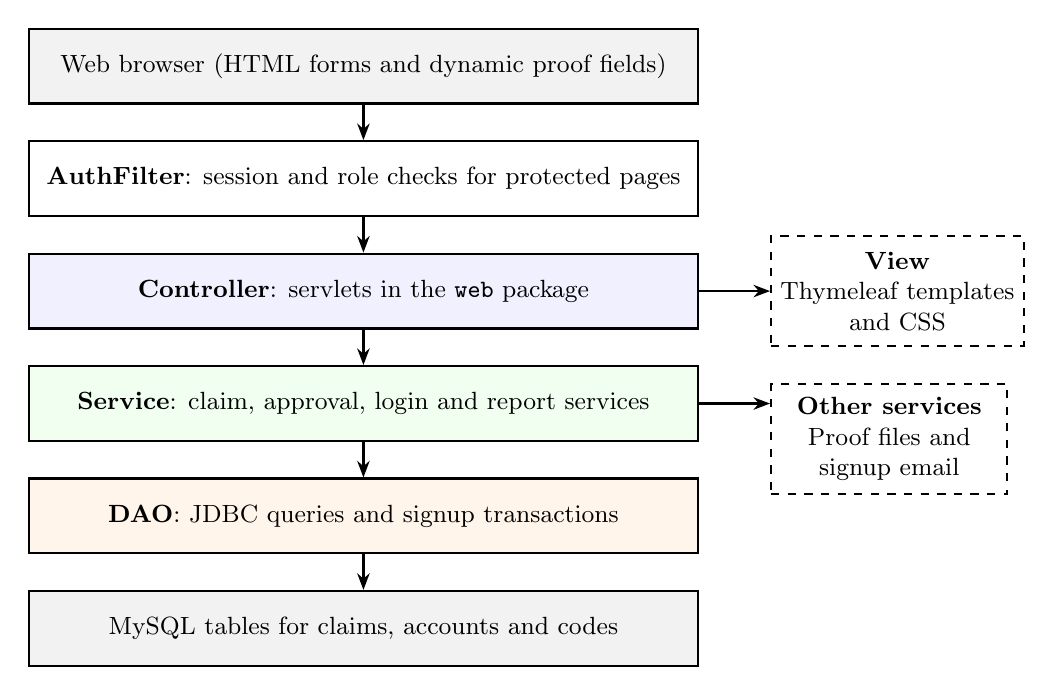
\begin{tikzpicture}[node distance=0.45cm]
  \node[layer,fill=gray!10] (browser) {Web browser (HTML forms and dynamic proof fields)};
  \node[layer,below=of browser] (filter) {\textbf{AuthFilter}: session and role checks for protected pages};
  \node[layer,below=of filter,fill=blue!6] (web) {\textbf{Controller}: servlets in the \texttt{web} package};
  \node[layer,below=of web,fill=green!6] (service) {\textbf{Service}: claim, approval, login and report services};
  \node[layer,below=of service,fill=orange!8] (dao) {\textbf{DAO}: JDBC queries and signup transactions};
  \node[layer,below=of dao,fill=gray!10] (db) {MySQL tables for claims, accounts and codes};

  \node[draw,thick,dashed,minimum width=3.0cm,minimum height=1.4cm,align=center,font=\small,right=0.9cm of web] (view) {\textbf{View}\\Thymeleaf templates\\and CSS};
  \node[draw,thick,dashed,minimum width=3.0cm,minimum height=1.4cm,align=center,font=\small,right=0.9cm of service,yshift=-0.45cm] (external) {\textbf{Other services}\\Proof files and\\signup email};

  \foreach \a/\b in {browser/filter,filter/web,web/service,service/dao,dao/db}
    \draw[uses] (\a) -- (\b);
  \draw[uses] (web) -- (view);
  \draw[uses] (service.east) -- (external.west |- service.east);
\end{tikzpicture}
\caption{Layered architecture of the system}
\label{fig:arch}
\end{figure}

\begin{itemize}
  \item \textbf{View:} Thymeleaf HTML templates in \texttt{WEB-INF/templates}. They only display data. The browser cannot open them directly.
  \item \textbf{Controller:} servlets read the form, call a service, and either redirect after success or show the page again with an error.
  \item \textbf{Service:} claim validation, lifecycle, escalation, report filtering, proof access and signup.
  \item \textbf{DAO:} JDBC classes use prepared statements for input values. Signup uses a transaction to create the student account and consume the code together.
  \item \textbf{Model:} plain Java objects shared by all layers.
\end{itemize}

\texttt{Main} starts embedded Apache Tomcat 10.1 on port 8080. Successful form submissions redirect to a fresh page. For a local demo, the command is \texttt{mvn compile exec:exec}.

\section{Use Case Diagram}

\begin{figure}[H]
\centering
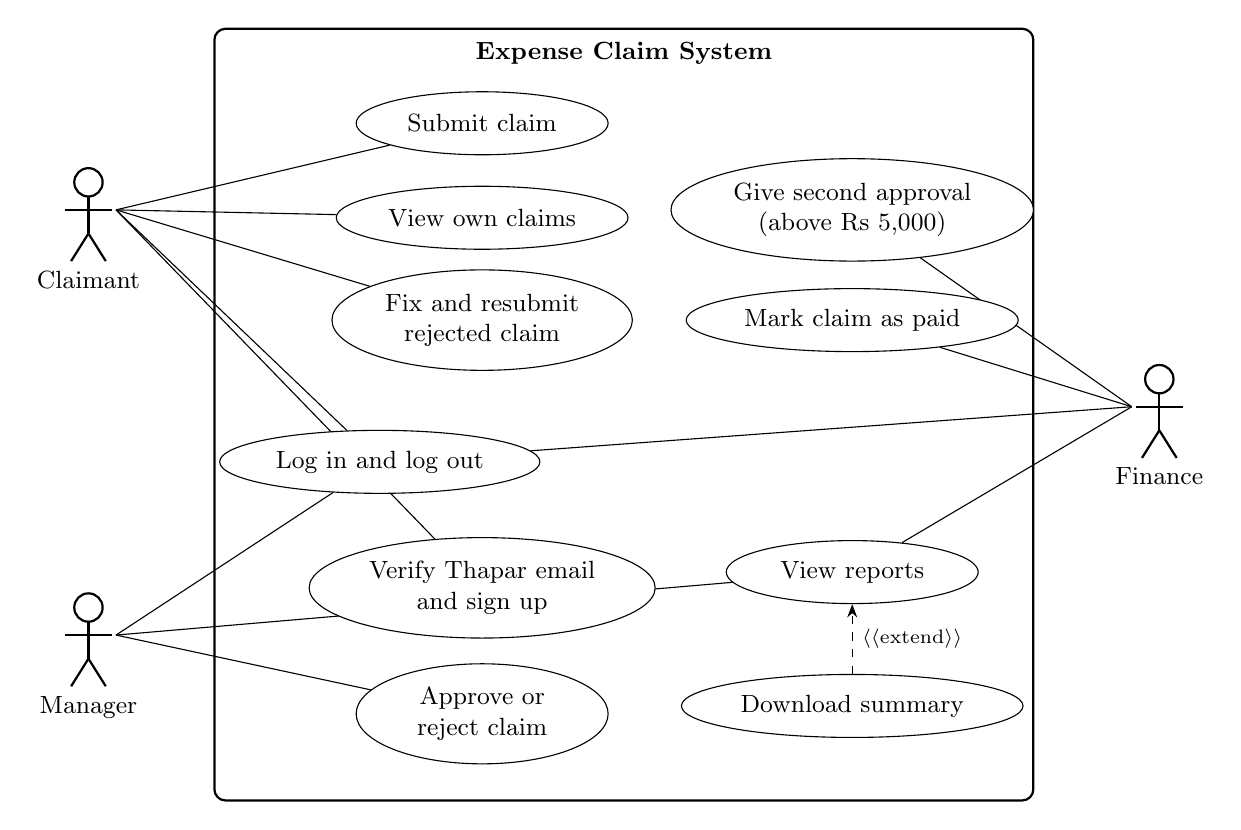
\begin{tikzpicture}
  \draw[thick,rounded corners=4pt] (1.6,-0.6) rectangle (12.0,9.2);
  \node[font=\small\bfseries,anchor=north] at (6.8,9.15) {Expense Claim System};

  \stickman{Claimant}{0}{6.3}
  \stickman{Manager}{0}{0.9}
  \stickman{Finance}{13.6}{3.8}
  \coordinate (emp) at (0.35,6.9);
  \coordinate (mgr) at (0.35,1.5);
  \coordinate (fin) at (13.25,4.4);

  \node[usecase] (submit) at (5.0,8.0) {Submit claim};
  \node[usecase] (own) at (5.0,6.8) {View own claims};
  \node[usecase] (fix) at (5.0,5.5) {Fix and resubmit\\rejected claim};
  \node[usecase] (signup) at (5.0,2.1) {Verify Thapar email\\and sign up};
  \node[usecase] (login) at (3.7,3.7) {Log in and log out};
  \node[usecase] (decide) at (5.0,0.5) {Approve or\\reject claim};
  \node[usecase] (second) at (9.7,6.9) {Give second approval\\(above Rs 5,000)};
  \node[usecase] (pay) at (9.7,5.5) {Mark claim as paid};
  \node[usecase] (reports) at (9.7,2.3) {View reports};
  \node[usecase] (download) at (9.7,0.6) {Download summary};

  \begin{pgfonlayer}{background}
    \foreach \u in {login,submit,own,fix,signup} \draw (emp) -- (\u);
    \foreach \u in {login,decide,reports} \draw (mgr) -- (\u);
    \foreach \u in {login,second,pay,reports} \draw (fin) -- (\u);
  \end{pgfonlayer}
  \draw[dashed,-{Stealth}] (download) -- node[right,font=\scriptsize]{$\langle\langle$extend$\rangle\rangle$} (reports);
\end{tikzpicture}
\caption{Use case diagram}
\label{fig:usecase}
\end{figure}

Claimants see their own claims. Managers act on their team's claims and confirm that they have checked the proof before approval. Finance sees claims in its own organisation and can give the second approval after the manager. Managers and finance can view and download reports within their permitted scope.

\section{Class Diagram}

Figure~\ref{fig:class-model} shows the model classes. \texttt{Claim} is abstract and declares \texttt{validate()}, \texttt{getType()} and \texttt{getLimit()}. Each subclass overrides them.

\begin{figure}[H]
\centering
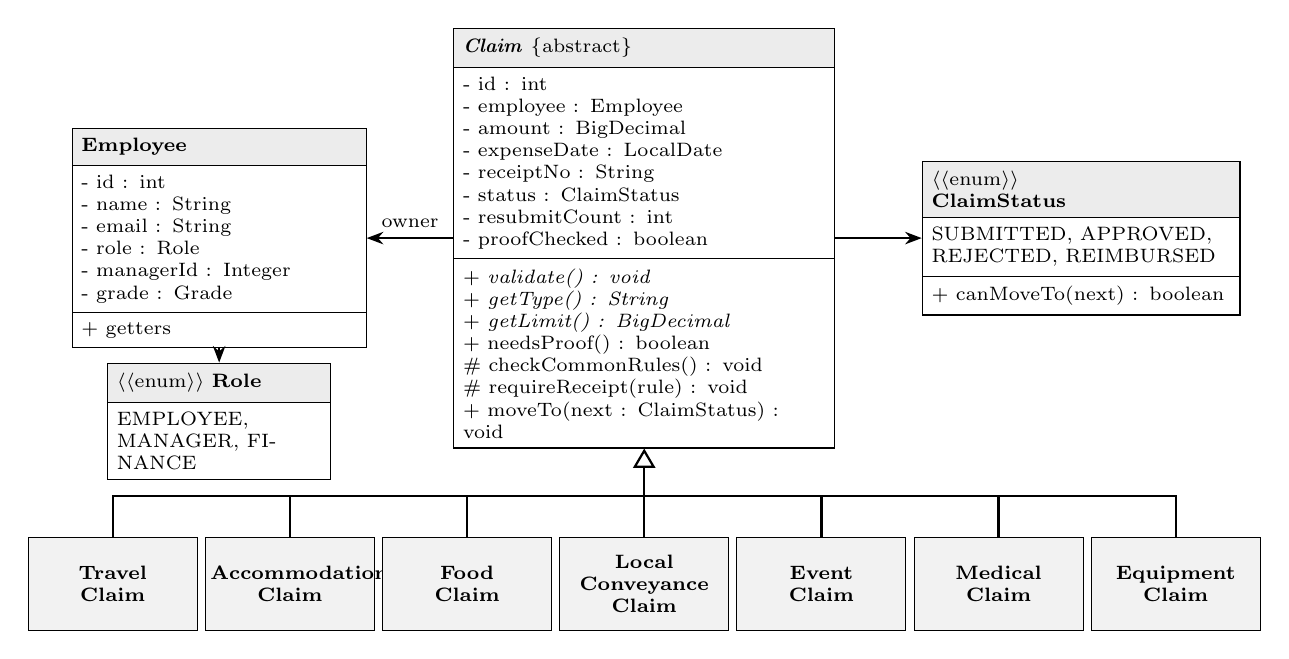
\begin{tikzpicture}[node distance=0.6cm and 0.5cm]
  \node[umlclass] (claim) {\textit{\textbf{Claim}} \{abstract\}
    \nodepart{second}
    - id : int\\
    - employee : Employee\\
    - amount : BigDecimal\\
    - expenseDate : LocalDate\\
    - receiptNo : String\\
    - status : ClaimStatus\\
    - resubmitCount : int\\
    - proofChecked : boolean
    \nodepart{third}
    + \textit{validate() : void}\\
    + \textit{getType() : String}\\
    + \textit{getLimit() : BigDecimal}\\
    + needsProof() : boolean\\
    \# checkCommonRules() : void\\
    \# requireReceipt(rule) : void\\
    + moveTo(next : ClaimStatus) : void};

  \node[umlclass,text width=3.5cm,left=1.1cm of claim] (emp) {\textbf{Employee}
    \nodepart{second}
    - id : int\\
    - name : String\\
    - email : String\\
    - role : Role\\
    - managerId : Integer\\
    - grade : Grade
    \nodepart{third}
    + getters};

  \node[umlclass,text width=3.8cm,right=1.1cm of claim] (status) {$\langle\langle$enum$\rangle\rangle$\\\textbf{ClaimStatus}
    \nodepart{second}
    SUBMITTED, APPROVED,\\ REJECTED, REIMBURSED
    \nodepart{third}
    + canMoveTo(next) : boolean};

  \node[umlsmall,text width=2.6cm,below=0.18cm of emp] (role) {$\langle\langle$enum$\rangle\rangle$ \textbf{Role}
    \nodepart{second} EMPLOYEE,\\ MANAGER, FINANCE};

  \coordinate (join) at ($(claim.south)+(0,-0.6)$);
  \draw[inherit] (join) -- (claim.south);
  \foreach \x/\name/\short in {-6.75/Travel/travel,-4.5/Accommodation/lodging,-2.25/Food/food,0/{Local\\Conveyance}/local,2.25/Event/event,4.5/Medical/medical,6.75/Equipment/equipment} {
    \node[draw,fill=gray!10,font=\scriptsize\bfseries,align=center,text width=2.02cm,inner sep=1.8pt,minimum height=1.18cm]
      (\short) at ($(join)+(\x,-1.12)$) {\name\\Claim};
    \draw[thick] (\short.north) |- (join);
  }

  \draw[uses] (claim.west) -- node[above,font=\scriptsize]{owner} (emp.east);
  \draw[uses] (claim.east) -- (status.west);
  \draw[uses] (emp.south) -- (role.north);
\end{tikzpicture}
\caption{Class diagram of the model package}
\label{fig:class-model}
\end{figure}

Figure~\ref{fig:class-service} shows the main service and data access classes. \texttt{ApprovalService} implements \texttt{Approvable}. The claim and approval services use DAO interfaces so unit tests can replace JDBC implementations with in-memory fakes. \texttt{SignupService} uses \texttt{JdbcSignupDAO} for account creation.

\begin{figure}[H]
\centering
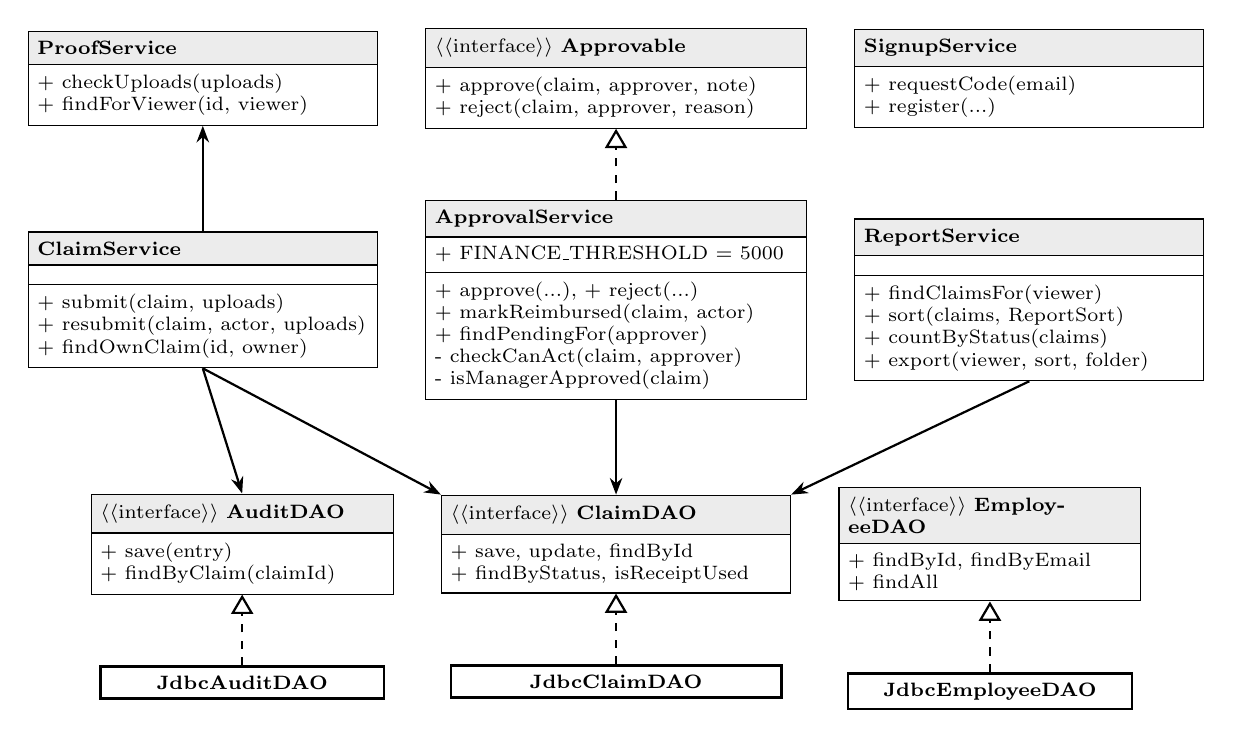
\begin{tikzpicture}[node distance=0.9cm and 0.6cm]
  \node[umlsmall,text width=4.6cm] (approvable) {$\langle\langle$interface$\rangle\rangle$ \textbf{Approvable}
    \nodepart{second} + approve(claim, approver, note)\\ + reject(claim, approver, reason)};
  \node[umlsmall,text width=4.2cm,left=0.6cm of approvable] (proofsvc) {\textbf{ProofService}
    \nodepart{second} + checkUploads(uploads)\\ + findForViewer(id, viewer)};
  \node[umlsmall,text width=4.2cm,right=0.6cm of approvable] (signupsvc) {\textbf{SignupService}
    \nodepart{second} + requestCode(email)\\ + register(...)};
  \node[umlclass,text width=4.6cm,below=0.9cm of approvable] (approval) {\textbf{ApprovalService}
    \nodepart{second} + FINANCE\_THRESHOLD = 5000
    \nodepart{third} + approve(...), + reject(...)\\ + markReimbursed(claim, actor)\\ + findPendingFor(approver)\\ - checkCanAct(claim, approver)\\ - isManagerApproved(claim)};
  \node[umlclass,text width=4.2cm,left=0.6cm of approval] (claimsvc) {\textbf{ClaimService}
    \nodepart{second} ~
    \nodepart{third} + submit(claim, uploads)\\ + resubmit(claim, actor, uploads)\\ + findOwnClaim(id, owner)};
  \node[umlclass,text width=4.2cm,right=0.6cm of approval] (report) {\textbf{ReportService}
    \nodepart{second} ~
    \nodepart{third} + findClaimsFor(viewer)\\ + sort(claims, ReportSort)\\ + countByStatus(claims)\\ + export(viewer, sort, folder)};

  \node[umlsmall,text width=4.2cm,below=1.2cm of approval] (claimdao) {$\langle\langle$interface$\rangle\rangle$ \textbf{ClaimDAO}
    \nodepart{second} + save, update, findById\\ + findByStatus, isReceiptUsed};
  \node[umlsmall,text width=3.6cm,left=0.6cm of claimdao] (auditdao) {$\langle\langle$interface$\rangle\rangle$ \textbf{AuditDAO}
    \nodepart{second} + save(entry)\\ + findByClaim(claimId)};
  \node[umlsmall,text width=3.6cm,right=0.6cm of claimdao] (empdao) {$\langle\langle$interface$\rangle\rangle$ \textbf{EmployeeDAO}
    \nodepart{second} + findById, findByEmail\\ + findAll};

  \node[draw,thick,font=\scriptsize,below=0.9cm of claimdao,minimum width=4.2cm] (jclaim) {\textbf{JdbcClaimDAO}};
  \node[draw,thick,font=\scriptsize,below=0.9cm of auditdao,minimum width=3.6cm] (jaudit) {\textbf{JdbcAuditDAO}};
  \node[draw,thick,font=\scriptsize,below=0.9cm of empdao,minimum width=3.6cm] (jemp) {\textbf{JdbcEmployeeDAO}};

  \draw[realize] (approval) -- (approvable);
  \draw[realize] (jclaim) -- (claimdao);
  \draw[realize] (jaudit) -- (auditdao);
  \draw[realize] (jemp) -- (empdao);
  \draw[uses] (approval.south) -- (claimdao.north);
  \draw[uses] (claimsvc.north) -- (proofsvc.south);
  \draw[uses] (claimsvc.south) -- (auditdao.north);
  \draw[uses] (claimsvc.south) -- (claimdao.north west);
  \draw[uses] (report.south) -- (claimdao.north east);
\end{tikzpicture}
\caption{Class diagram of the service and DAO layers}
\label{fig:class-service}
\end{figure}

\section{Activity Diagram}

Figure~\ref{fig:activity} shows the full lifecycle of a claim, including rejection, resubmission and the second approval by finance.

\begin{figure}[H]
\centering
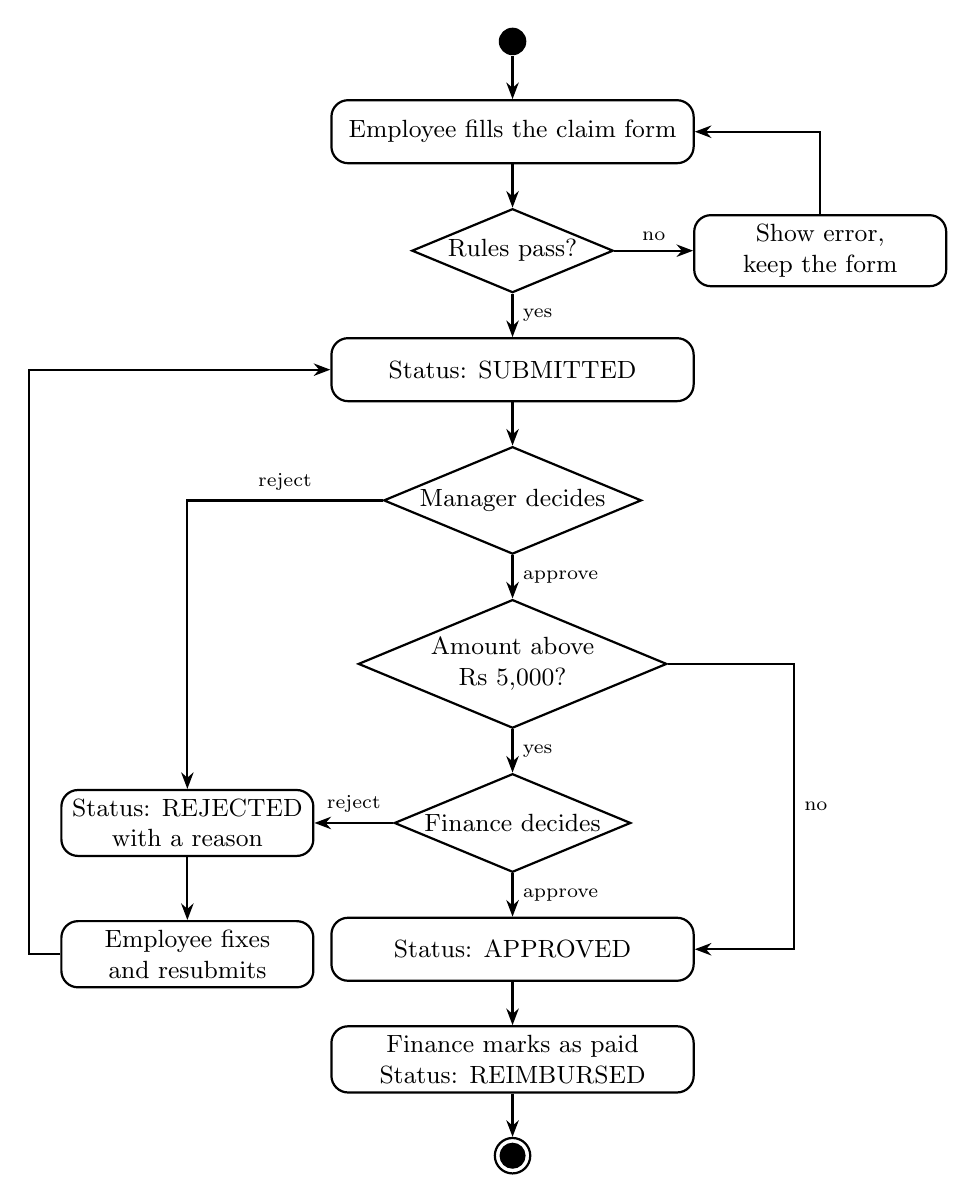
\begin{tikzpicture}[node distance=0.55cm]
  \node[circle,fill=black,minimum size=0.35cm] (start) {};
  \node[flowstep,below=of start] (fill) {Employee fills the claim form};
  \node[choice,below=of fill] (valid) {Rules pass?};
  \node[flowstep,below=of valid] (sub) {Status: SUBMITTED};
  \node[choice,below=of sub] (mgr) {Manager decides};
  \node[choice,below=of mgr] (big) {Amount above\\Rs 5,000?};
  \node[choice,below=of big] (fin) {Finance decides};
  \node[flowstep,below=of fin] (app) {Status: APPROVED};
  \node[flowstep,below=of app] (paid) {Finance marks as paid\\Status: REIMBURSED};
  \node[circle,draw,thick,minimum size=0.45cm,below=of paid] (end) {};
  \node[circle,fill=black,minimum size=0.25cm] at (end) {};

  \node[flowstep,minimum width=3.2cm,right=1.0cm of valid] (err) {Show error,\\keep the form};
  \node[flowstep,minimum width=3.2cm,left=1.0cm of fin] (rej) {Status: REJECTED\\with a reason};
  \node[flowstep,minimum width=3.2cm,below=0.8cm of rej] (fix) {Employee fixes\\and resubmits};

  \draw[uses] (start) -- (fill);
  \draw[uses] (fill) -- (valid);
  \draw[uses] (valid) -- node[right,font=\scriptsize]{yes} (sub);
  \draw[uses] (valid) -- node[above,font=\scriptsize]{no} (err);
  \draw[uses] (err) |- (fill);
  \draw[uses] (sub) -- (mgr);
  \draw[uses] (mgr) -- node[right,font=\scriptsize]{approve} (big);
  \draw[uses] (mgr.west) -| node[pos=0.25,above,font=\scriptsize]{reject} (rej.north);
  \draw[uses] (big) -- node[right,font=\scriptsize]{yes} (fin);
  \draw[uses] (big.east) -- ++(1.6,0) |- node[pos=0.25,right,font=\scriptsize]{no} (app.east);
  \draw[uses] (fin) -- node[right,font=\scriptsize]{approve} (app);
  \draw[uses] (fin.west) -- node[above,font=\scriptsize]{reject} (rej.east);
  \draw[uses] (rej) -- (fix);
  \draw[uses] (fix.west) -- ++(-0.4,0) |- (sub.west);
  \draw[uses] (app) -- (paid);
  \draw[uses] (paid) -- (end);
\end{tikzpicture}
\caption{Activity diagram of the claim lifecycle}
\label{fig:activity}
\end{figure}

The allowed moves are SUBMITTED to APPROVED or REJECTED, APPROVED to REIMBURSED, and REJECTED back to SUBMITTED. REIMBURSED is final. A manager approval of a claim above Rs 5,000 does not change its status. It is recorded as an audit row from SUBMITTED to SUBMITTED, and the claim waits for finance.

\section{Database Design / ER Diagram}

Figure~\ref{fig:er} shows the five tables used by the current application.

\begin{figure}[H]
\centering
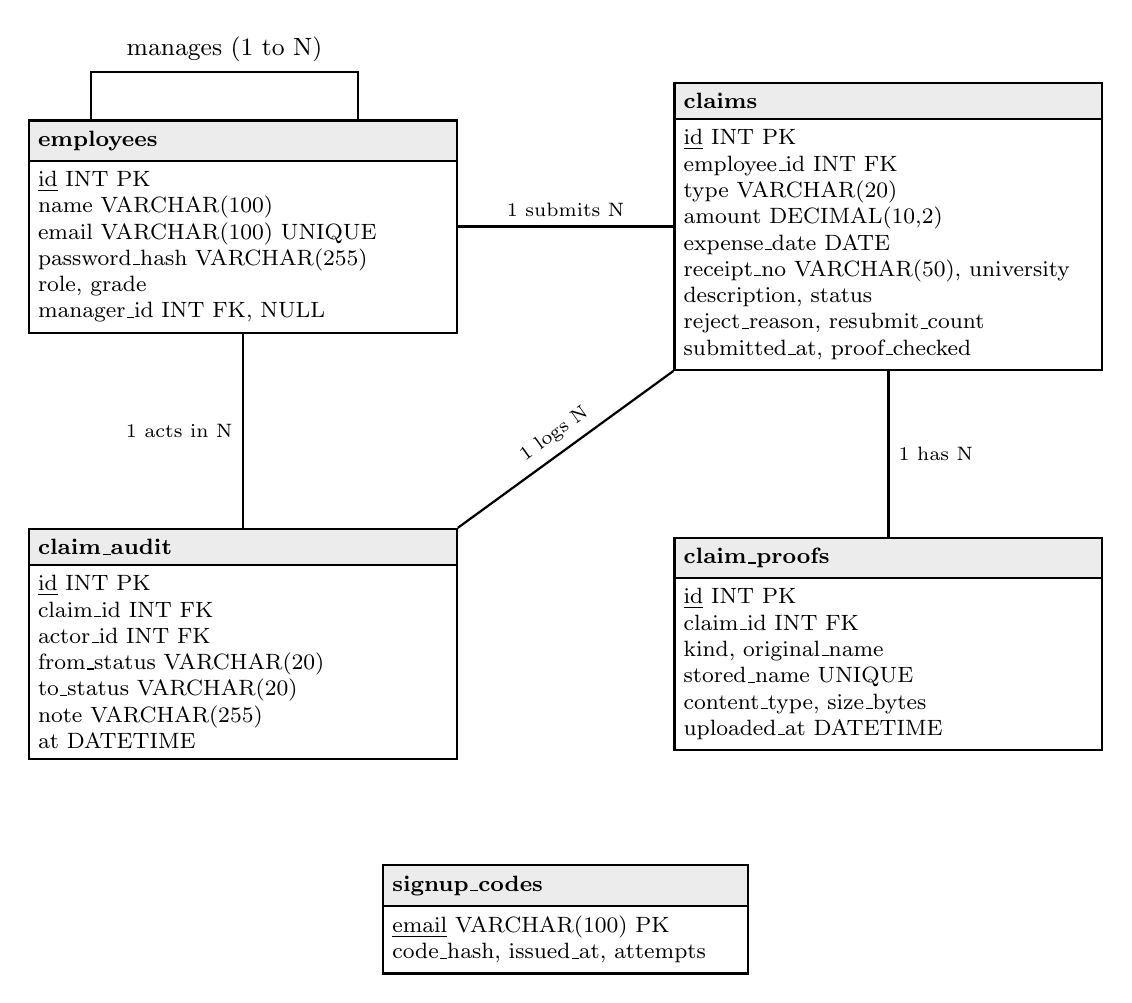
\begin{tikzpicture}
  \node[entity] (emp) at (0,0) {\textbf{employees}
    \nodepart{second}
    \underline{id} INT PK\\
    name VARCHAR(100)\\
    email VARCHAR(100) UNIQUE\\
    password\_hash VARCHAR(255)\\
    role, grade\\
    manager\_id INT FK, NULL};
  \node[entity] (claims) at (8.2,0) {\textbf{claims}
    \nodepart{second}
    \underline{id} INT PK\\
    employee\_id INT FK\\
    type VARCHAR(20)\\
    amount DECIMAL(10,2)\\
    expense\_date DATE\\
    receipt\_no VARCHAR(50), university\\
    description, status\\
    reject\_reason, resubmit\_count\\
    submitted\_at, proof\_checked};
  \node[entity] (audit) at (0,-5.3) {\textbf{claim\_audit}
    \nodepart{second}
    \underline{id} INT PK\\
    claim\_id INT FK\\
    actor\_id INT FK\\
    from\_status VARCHAR(20)\\
    to\_status VARCHAR(20)\\
    note VARCHAR(255)\\
    at DATETIME};
  \node[entity] (proof) at (8.2,-5.3) {\textbf{claim\_proofs}
    \nodepart{second}
    \underline{id} INT PK\\
    claim\_id INT FK\\
    kind, original\_name\\
    stored\_name UNIQUE\\
    content\_type, size\_bytes\\
    uploaded\_at DATETIME};
  \node[entity,text width=4.4cm] at (4.1,-8.8) {\textbf{signup\_codes}
    \nodepart{second}
    \underline{email} VARCHAR(100) PK\\
    code\_hash, issued\_at, attempts};

  \draw[thick] (emp.east) -- node[above,font=\scriptsize]{1 submits N} (claims.west);
  \draw[thick] (emp.south) -- node[left,font=\scriptsize]{1 acts in N} (audit.north);
  \draw[thick] (claims.south) -- node[right,font=\scriptsize]{1 has N} (proof.north);
  \draw[thick] (claims.south west) -- node[above,sloped,font=\scriptsize]{1 logs N} (audit.north east);
  \draw[thick] ([xshift=0.8cm]emp.north west) -- ++(0,0.6) -- node[above,font=\small]{manages (1 to N)} ++(3.4,0) -- ++(0,-0.6);
\end{tikzpicture}
\caption{ER diagram}
\label{fig:er}
\end{figure}

\begin{itemize}
  \item \texttt{employees.manager\_id} points to another employee, so the table stores the reporting line.
  \item A unique index on \texttt{(university, receipt\_no)} prevents reusing a receipt within an organisation. Claims that do not need a receipt can store NULL.
  \item \texttt{claim\_audit} stores decisions and their actors. \texttt{claim\_proofs} stores file names and metadata. The files themselves live in \texttt{uploads/}.
  \item \texttt{signup\_codes} tracks pending verification before an employee record exists. New accounts use salted PBKDF2 password hashes. The SHA-256 hashes in the seed data are for the local demo.
\end{itemize}

\section{Module Description}

\begin{description}[style=nextline,leftmargin=0.6cm]
  \item[Login and signup module] Checks credentials, starts a new \texttt{HttpSession}, and routes users by role. Thapar signup verifies an email code and creates a student account assigned to a reviewer.
  \item[Claim module] Lets an employee submit a claim, see all their claims with a progress bar, and fix and resubmit a rejected claim. Every claim is validated by its own subclass, and duplicate receipts are blocked.
  \item[Approval module] Lets a manager approve or reject the claims of their team, and finance give the second approval and mark claims as paid. It stops self approval, approval by the wrong manager and illegal status moves.
  \item[Audit module] Writes one \texttt{claim\_audit} row for every submission, approval, rejection, resubmission and payment.
  \item[Proof module] Validates file size and signature, saves the file under a random name, and checks whether the viewer may open it.
  \item[Report module] Shows claims sorted by date, amount or status, with the count and total for each status, and writes a summary text file that the browser downloads.
\end{description}

% ---------------- Chapter 3 ----------------
\chapter{Implementation}

\section{Technologies and Tools Used}

\begin{table}[H]
\centering
\begin{singlespace}
\begin{tabularx}{\linewidth}{>{\bfseries}l Y}
\toprule
Technology & Use in the project\\
\midrule
Java 21 & Source language and runtime\\
Jakarta Servlet 6.0 & HTTP controllers, filters and startup listeners\\
Apache Tomcat 10.1 (embedded) & Web server started from \texttt{Main} on port 8080\\
Thymeleaf 3.1 & HTML templates for the pages\\
MySQL 8.0 & Stores accounts, claims, proof metadata, audit rows and signup codes\\
JDBC (MySQL Connector/J 8.4) & Database access through \texttt{PreparedStatement}\\
JUnit 5 & 132 unit and integration tests\\
Maven & Build, dependencies, running tests and starting the server\\
HTML, CSS and JavaScript & Page layout, styling and dynamic proof fields\\
Resend & Optional delivery of Thapar signup codes\\
Git and GitHub & Version control\\
\bottomrule
\end{tabularx}
\end{singlespace}
\caption{Technologies and tools}
\end{table}

\section{Project Structure / Package Structure}

\begin{lstlisting}[language={}]
src/main/java/com/reimbursement
  Main.java       Embedded Tomcat startup
  model/          Claim subclasses, Employee, proof and audit records, enums
  exception/      Checked business and data-access exceptions
  dao/            DAO interfaces, DBConnection and JDBC implementations
  service/        Claim, approval, login, signup, proof and reporting services
  web/            Servlets, AuthFilter, Views, ClaimForm and Messages
  util/           AppContext, file storage, report writing and email delivery
src/main/webapp
  WEB-INF/        Thymeleaf pages, shared fragments and servlet configuration
  css/, js/       Styles and dynamic proof fields
src/test/java/    JUnit unit and integration tests
sql/              Schema, demo accounts and migration scripts
\end{lstlisting}

\section{Description of Classes and Interfaces}

\begin{table}[H]
\centering
\small
\begin{tabularx}{\linewidth}{>{\raggedright\arraybackslash\ttfamily}p{5.0cm} Y}
\toprule
\normalfont\bfseries Class or interface & \bfseries Purpose\\
\midrule
Claim (abstract) & Common fields of a claim, the shared rules in \texttt{checkCommonRules()}, and the lifecycle move \texttt{moveTo()}\\
EquipmentClaim, EventClaim & Apply the rules for Company purchases and student academic expenses\\
ClaimStatus (enum) & The four statuses and the allowed moves in \texttt{canMoveTo()}\\
Role (enum) & EMPLOYEE, MANAGER and FINANCE\\
Employee & Stores the user's grade, role and manager and identifies the organisation from the email\\
ClaimFactory & Builds a claim from its type and supplies the allowed types for a claimant\\
Approvable (interface) & Declares \texttt{approve()} and \texttt{reject()}\\
ApprovalService & Implements \texttt{Approvable}: escalation, authority checks, self approval, payment\\
ClaimService & Submit and resubmit with validation, duplicate receipt check and audit rows\\
LoginService, Passwords & Check credentials and hash new passwords with PBKDF2\\
SignupService, JdbcSignupDAO & Verify email codes and create student accounts in a transaction\\
ProofService, ProofStore & Check and store uploads and control who can open them\\
ReportService, ReportSort & Filter by organisation and role, sort, count, total and export claims\\
ClaimDAO, AuditDAO, ProofDAO & Interfaces for claim, audit and proof access\\
DBConnection & Opens JDBC connections using environment variables or local \texttt{db.properties}\\
ReportWriter & Writes the summary report with \texttt{FileWriter}\\
AuthFilter & Servlet filter for login and role checks\\
ApprovalServlet (abstract) & Shared approve and reject handling, extended by ManagerServlet and FinanceServlet\\
Views & Builds the Thymeleaf engine at startup and renders pages\\
ReimbursementException & Checked base class of all custom exceptions\\
\bottomrule
\end{tabularx}
\caption{Main classes and interfaces}
\end{table}

\section{Implementation of Major Modules}

\subsection*{Claim validation}
\texttt{Claim.checkCommonRules()} checks the rules shared by every type: the amount must be above zero with at most two decimal places, the text fields must fit their columns, the expense date must not be in the future or older than 60 days, and the amount must not be above \texttt{getLimit()}. The base class calls the abstract \texttt{getLimit()}, and Java picks the subclass version at run time. Each subclass then adds its own receipt rule.

\begin{table}[H]
\centering
\small
\begin{tabularx}{\linewidth}{>{\raggedright\arraybackslash}p{3.5cm} r r Y}
\toprule
Expense type & Student (Rs) & Company (Rs) & Required proof\\
\midrule
Travel & 6,000 & 25,000 & Ticket or boarding pass\\
Accommodation & 2,500 & 12,000 & Accommodation invoice\\
Food and meals & 1,500 & 2,000 & Itemised bill for students above Rs 200. Company meals are an allowance.\\
Local transport & 800 & 3,000 & Transit receipt above Rs 200\\
Academic events and materials & 10,000 & N/A & Fee receipt or bill\\
Equipment and electronics & N/A & 25,000 & Purchase invoice\\
Medical & 50,000 & 50,000 & Medical bill or prescription\\
\bottomrule
\end{tabularx}
\caption{Claim limits and proof requirements}
\end{table}

When proof is required, the claimant enters the receipt number and uploads a file. Student travel and academic events can include an optional HoD or Dean letter alongside the required proof. The equipment description can identify the item and model.

\subsection*{Lifecycle and escalation}
\texttt{ClaimStatus.canMoveTo()} lists the four allowed moves. \texttt{ApprovalService.approve()} checks the actor's organisation, authority and the claim's status. For a claim with an uploaded document, the manager must select \textbf{Proof checked}. Above Rs 5,000, the claim remains submitted after manager approval and an audit row records that it is waiting for finance. Resubmission clears the proof check and requires a new decision.

\subsection*{Login and access control}
\texttt{LoginServlet} checks the credentials through \texttt{LoginService} and creates a fresh session. \texttt{AuthFilter} checks access by role, and the services check organisation and ownership when opening a claim, approving it, viewing proof or exporting reports.

\subsection*{Student signup and proof uploads}
Registration accepts an \texttt{@thapar.edu} address when a mail sender and reviewer are configured. The email contains a six-digit code. The server stores a keyed hash of the code, expires it after ten minutes and limits failed attempts. Verification creates a student account and consumes the code in the same database transaction.

The form accepts PDF, JPEG, PNG and WEBP proof files up to 5 MB each, with at most two files per claim. \texttt{ProofService} checks the file signature, and \texttt{ProofStore} saves the file in \texttt{uploads/} under a random name. The database retains the file metadata and claim link.

\subsection*{Claim pages}
\texttt{EmployeeServlet} uses \texttt{ClaimForm} to turn the text fields into a \texttt{BigDecimal}, a \texttt{LocalDate} and a claim id. \texttt{ClaimService.findOwnClaim()} checks the owner every time a claim is loaded, so changing the claim id in the URL cannot open another person's claim. \texttt{ManagerServlet} and \texttt{FinanceServlet} extend the abstract \texttt{ApprovalServlet}. Finance overrides \texttt{handle()} to add the payment action.

\subsection*{Reports}
\texttt{ReportService} filters claims by organisation and role. The servlet sorts them with the \texttt{Comparator} held by \texttt{ReportSort} and shows totals by status. The download servlet sends the summary written by \texttt{ReportWriter} as an attachment.

\section{Exception Handling}

All business rules are reported with custom \textbf{checked} exceptions. Each one extends the base class \texttt{ReimbursementException}, and that class extends \texttt{Exception}. Because they are checked, the compiler forces every caller to handle them.

\begin{figure}[H]
\centering
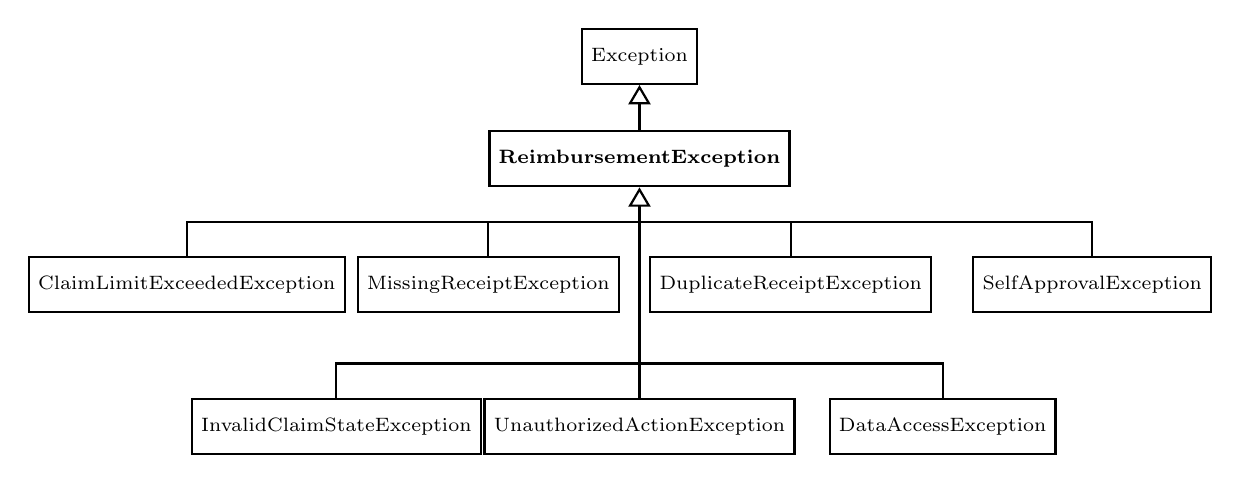
\begin{tikzpicture}[every node/.style={draw,thick,font=\scriptsize,minimum height=0.7cm,align=center,fill=white}]
  \node (ex) at (0,0) {Exception};
  \node (base) at (0,-1.3) {\textbf{ReimbursementException}};
  \node (a) at (-5.75,-2.9) {ClaimLimitExceededException};
  \node (b) at (-1.92,-2.9) {MissingReceiptException};
  \node (c) at (1.92,-2.9) {DuplicateReceiptException};
  \node (d) at (5.75,-2.9) {SelfApprovalException};
  \node (e) at (-3.85,-4.7) {InvalidClaimStateException};
  \node (f) at (0,-4.7) {UnauthorizedActionException};
  \node (g) at (3.85,-4.7) {DataAccessException};
  \draw[inherit] (base) -- (ex);
  \coordinate (j) at (0,-2.1);
  \coordinate (k) at (0,-3.9);
  \draw[inherit] (j) -- (base);
  \foreach \n in {a,b,c,d} \draw[thick] (\n.north) |- (j);
  \draw[thick] (k) -- (j);
  \foreach \n in {e,g} \draw[thick] (\n.north) |- (k);
  \draw[thick] (f.north) -- (k);
\end{tikzpicture}
\caption{Custom exception hierarchy}
\end{figure}

\begin{itemize}
  \item \textbf{Rule exceptions} are thrown by the model and service classes, for example when a claim is above its limit or a manager tries to approve the claim of another team.
  \item \textbf{DataAccessException} wraps every \texttt{SQLException} in the DAO layer and keeps it as the cause, so no JDBC type leaks into the services.
  \item \textbf{In the web layer}, servlets catch the base class \texttt{ReimbursementException}. The method \texttt{Messages.describe()} then uses a pattern matching \texttt{switch} on the exception type to add a short heading such as ``Over the limit'' or ``Not allowed''. The page is shown again with the message and the user's input kept.
  \item Bad input is caught in \texttt{ClaimForm} and turned into a clear message. A text amount throws \texttt{NumberFormatException}, and a badly formed date throws \texttt{DateTimeParseException}.
\end{itemize}

\lstinputlisting[firstline=3,lastline=8,caption={A custom checked exception}]{\src{exception/ClaimLimitExceededException.java}}

\section{Collection Framework Usage}

\begin{table}[H]
\centering
\small
\begin{tabularx}{\linewidth}{>{\ttfamily}l Y}
\toprule
\normalfont\bfseries Collection & \bfseries Where and why\\
\midrule
ArrayList<Claim> & Lists of claims returned by the DAOs and shown in tables\\
ConcurrentHashMap<Integer, Employee> & Cache in \texttt{JdbcEmployeeDAO}, so each employee is loaded once. It is thread safe because Tomcat serves many requests at the same time\\
HashMap & In-memory fake DAO used by the service tests\\
EnumMap<ClaimStatus, Integer> & Count and total of claims for each status in reports, kept in lifecycle order\\
Map<String, Set<Role>> with EnumSet & Which roles may open which path in \texttt{AuthFilter}\\
Comparator<Claim> & Sorting in reports, built with \texttt{comparing()}, \texttt{reversed()} and \texttt{thenComparing()}\\
Optional<Claim>, Optional<Employee> & Returned by DAO find methods instead of \texttt{null}\\
\bottomrule
\end{tabularx}
\caption{Collections used in the project}
\end{table}

\lstinputlisting[firstline=7,lastline=12,caption={Each sort option holds its own Comparator}]{\src{service/ReportSort.java}}

\lstinputlisting[firstline=57,lastline=66,caption={Counting claims per status with an EnumMap}]{\src{service/ReportService.java}}

\section{Database Connectivity}

\texttt{DBConnection} reads credentials from environment variables for hosted use or from the ignored local \texttt{db.properties} file. It opens a connection with \texttt{DriverManager}. The DAO methods use try-with-resources and bind input values through \texttt{PreparedStatement}.

\lstinputlisting[firstline=17,lastline=28,caption={Opening a connection from runtime variables or local settings}]{\src{dao/DBConnection.java}}

\lstinputlisting[firstline=41,lastline=66,caption={Saving a claim and reading back its generated id}]{\src{dao/jdbc/JdbcClaimDAO.java}}

\section{Important Code Snippets}

\lstinputlisting[firstline=3,lastline=17,caption={The claim lifecycle in the ClaimStatus enum}]{\src{model/ClaimStatus.java}}

\lstinputlisting[firstline=70,lastline=98,caption={Rules shared by every claim type in the abstract Claim class}]{\src{model/Claim.java}}

\lstinputlisting[firstline=17,lastline=21,caption={EquipmentClaim requires a purchase invoice number}]{\src{model/EquipmentClaim.java}}

\lstinputlisting[firstline=7,lastline=12,caption={The Approvable interface}]{\src{service/Approvable.java}}

\lstinputlisting[firstline=43,lastline=67,caption={Manager approval checks proof and records escalation}]{\src{service/ApprovalService.java}}

\lstinputlisting[firstline=33,lastline=56,caption={AuthFilter checks login and role before every request}]{\src{web/AuthFilter.java}}

% ---------------- Chapter 4 ----------------
\chapter{Results and Screenshots}

The results use demo accounts and sample claims. The claim pages show what an employee, reviewer or finance user can access in their own organisation.

\section{Main Application Screen}

\begin{figure}[H]
\centering
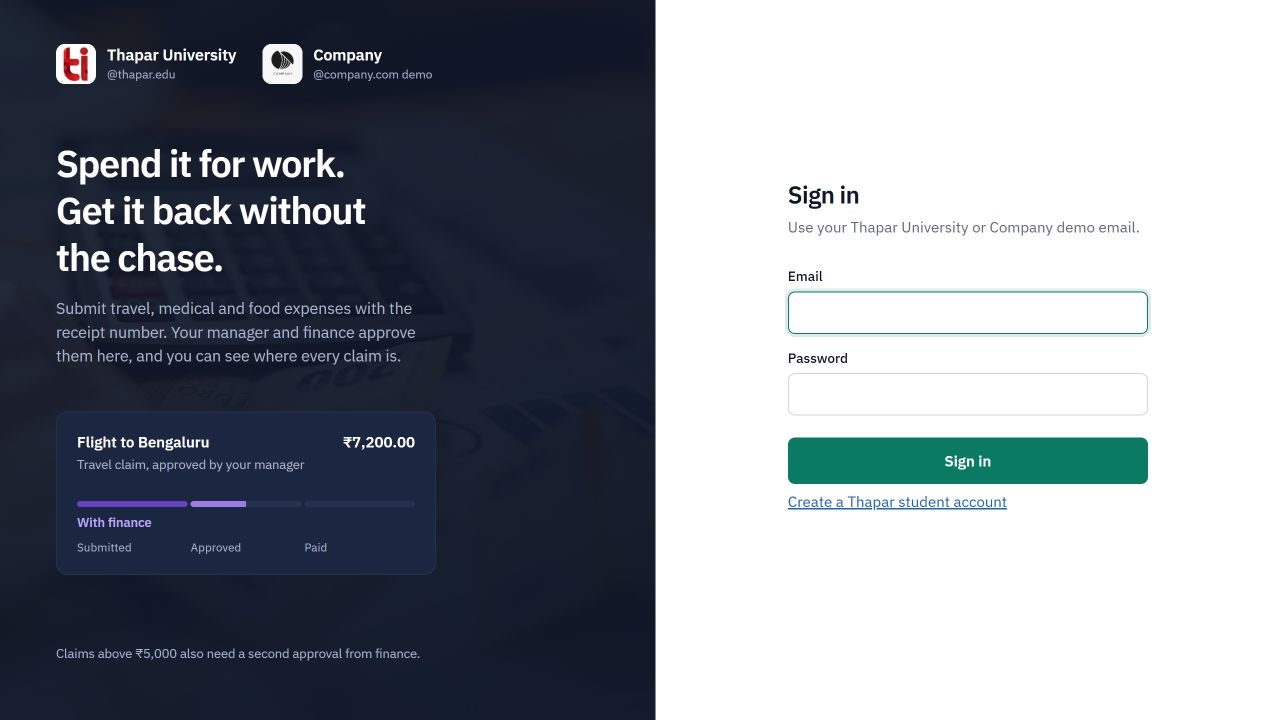
\includegraphics[width=\linewidth]{images/current-login.jpg}
\caption{Sign-in page for Thapar University and the Company demo}
\end{figure}

\begin{figure}[H]
\centering
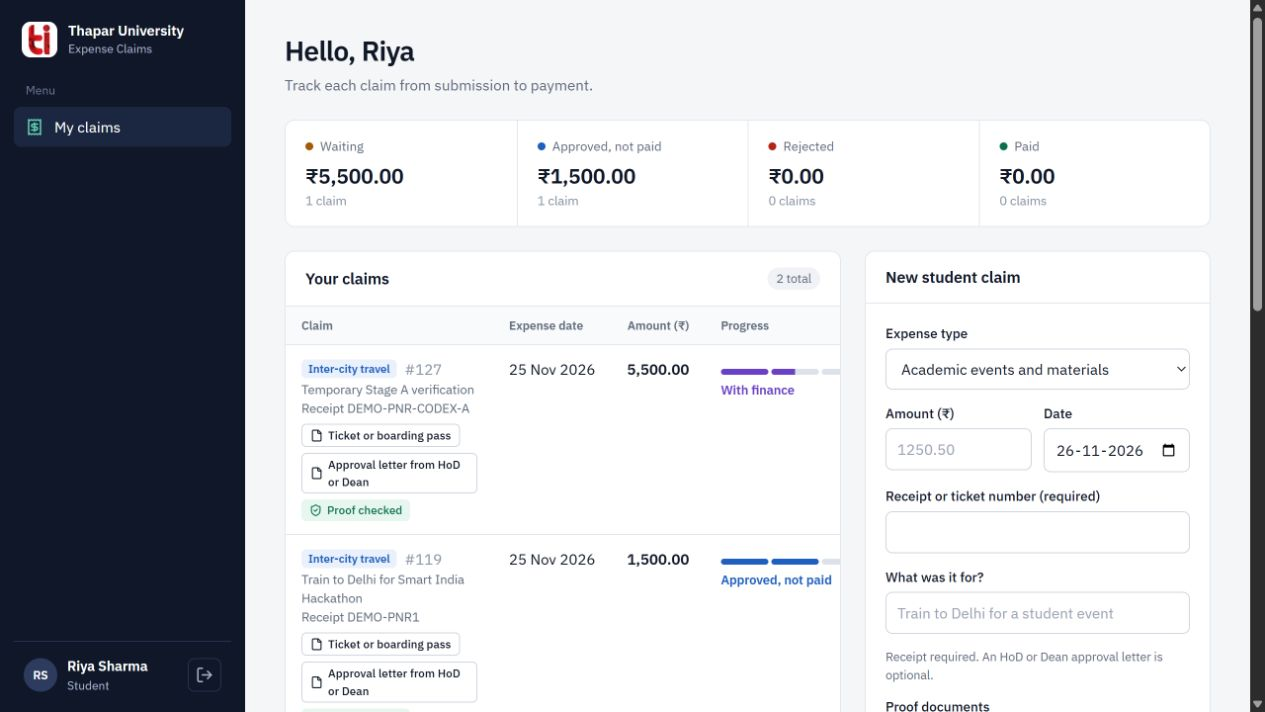
\includegraphics[width=\linewidth]{images/current-student.jpg}
\caption{Thapar claim page with the academic events form and optional approval letter}
\end{figure}

The employee page lists the employee's claims with a progress bar of three steps: submitted, approved and paid. A rejected claim shows the reason and a button to fix and resend it.

\section{Functional Screenshots}

\begin{figure}[H]
\centering
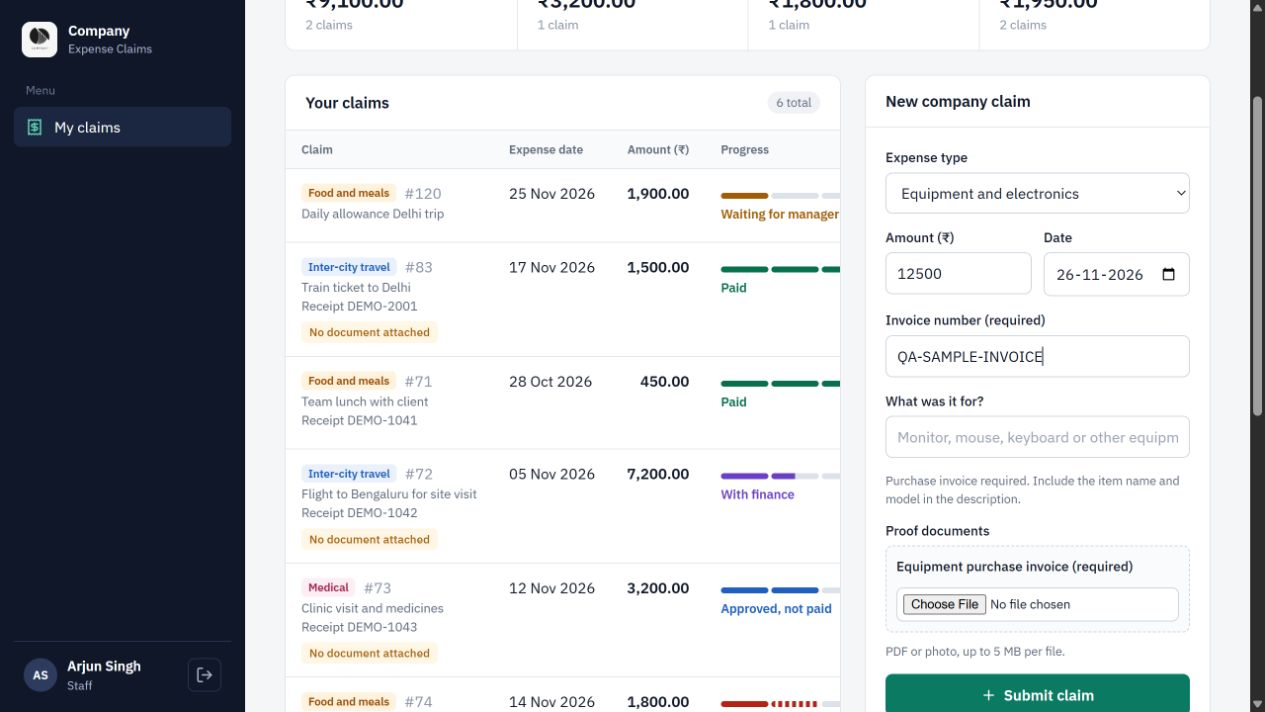
\includegraphics[width=\linewidth]{images/current-equipment.jpg}
\caption{Company equipment claim for a monitor, with a purchase invoice field}
\end{figure}

\begin{figure}[H]
\centering
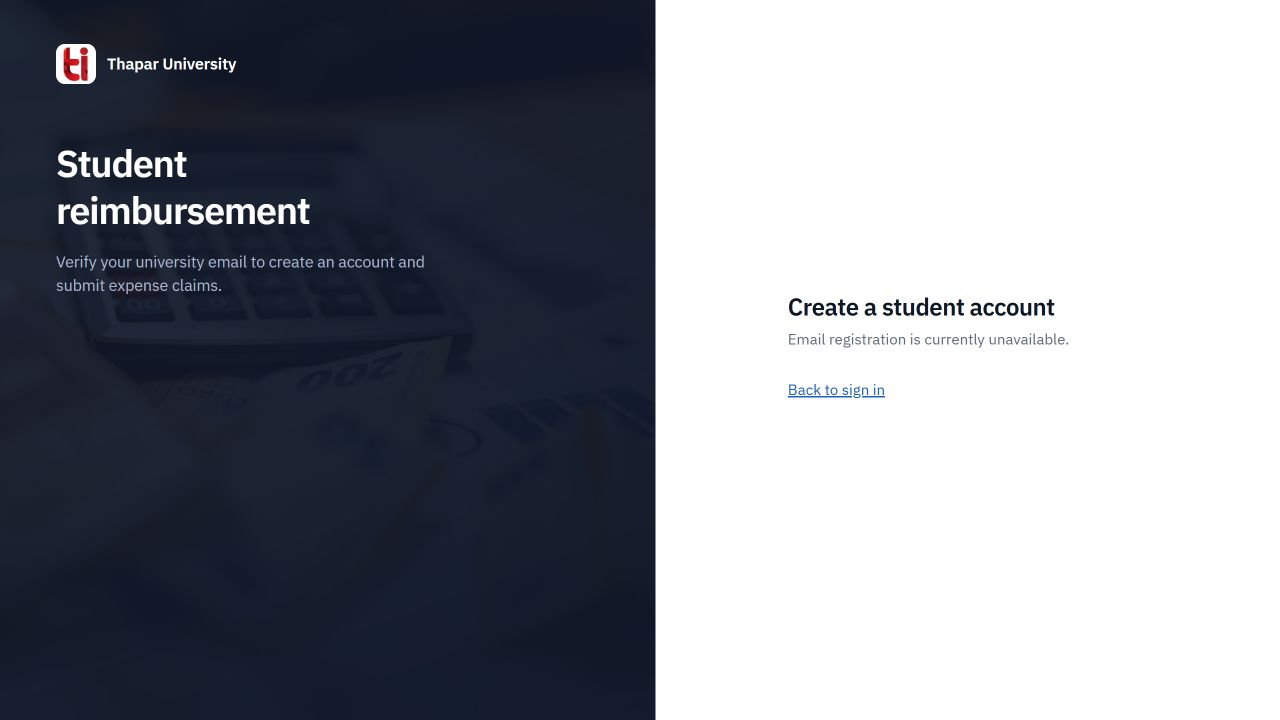
\includegraphics[width=\linewidth]{images/current-signup.jpg}
\caption{Thapar signup page in the local demo, where email delivery is disabled}
\end{figure}

\begin{figure}[H]
\centering
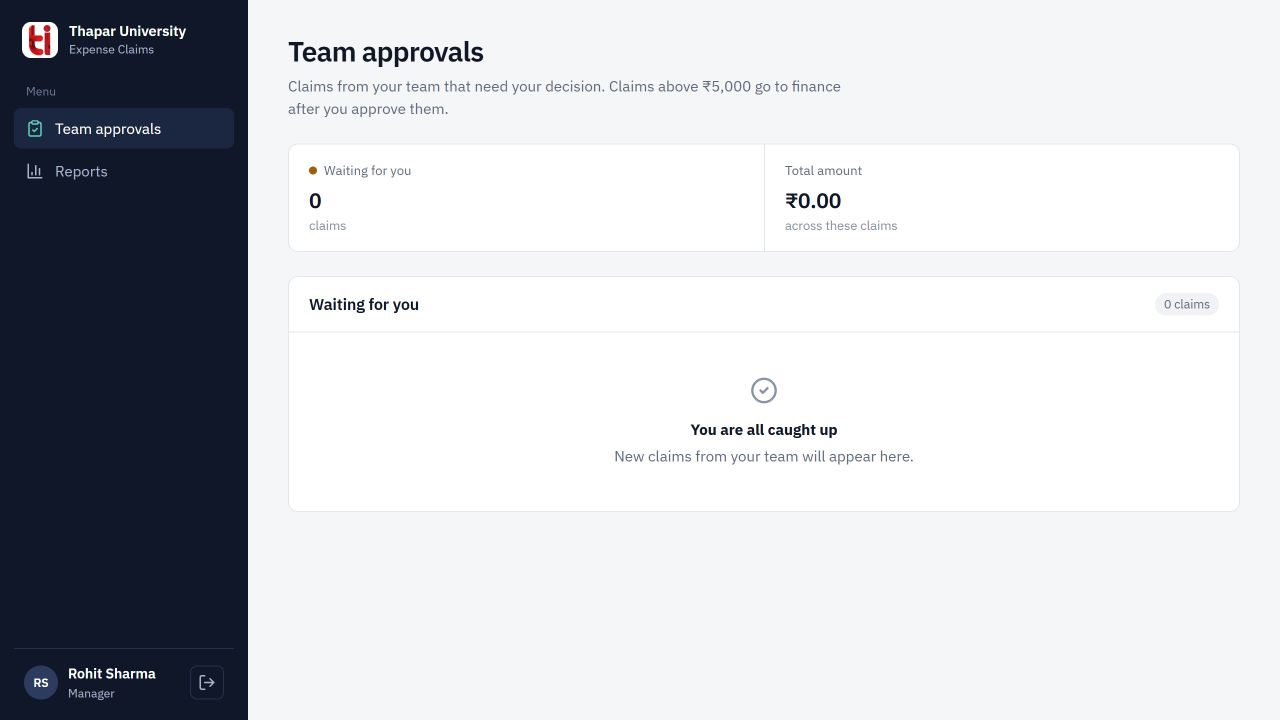
\includegraphics[width=\linewidth]{images/current-manager.jpg}
\caption{Thapar reviewer page showing the queue for their team}
\end{figure}

\begin{figure}[H]
\centering
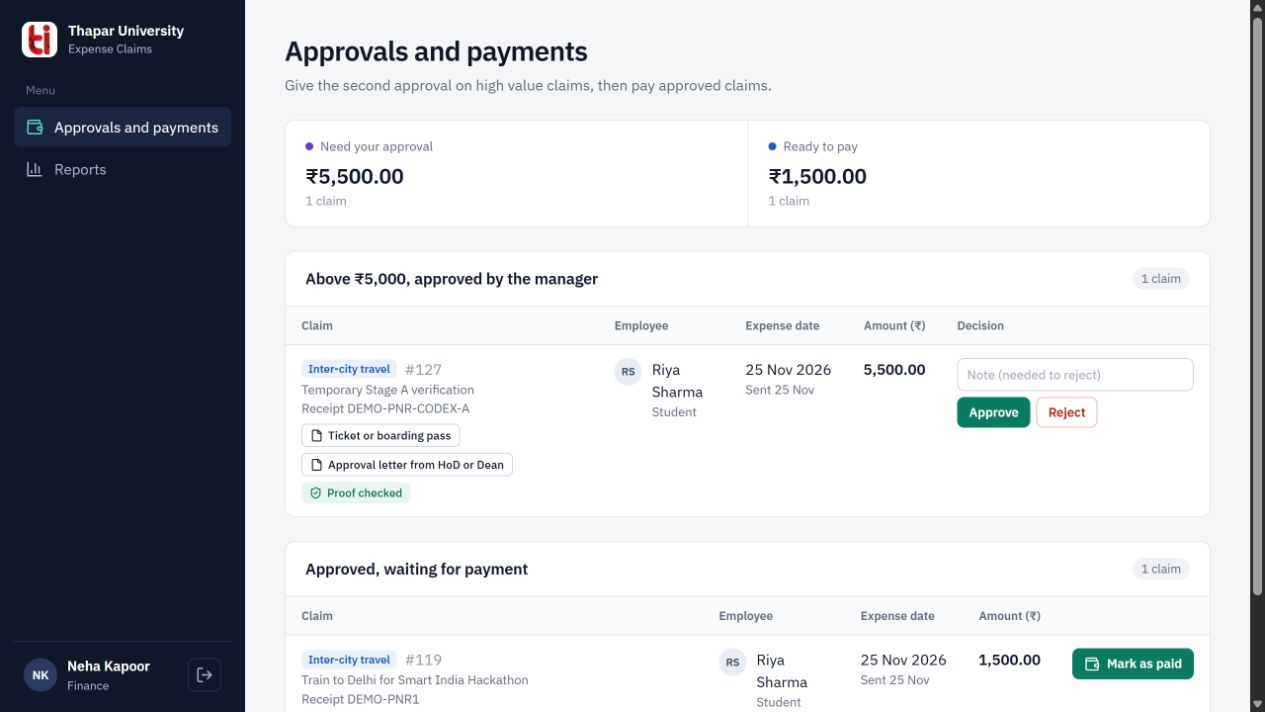
\includegraphics[width=\linewidth]{images/current-finance.jpg}
\caption{Thapar finance queue with the second approval and payment lists}
\end{figure}

\begin{figure}[H]
\centering
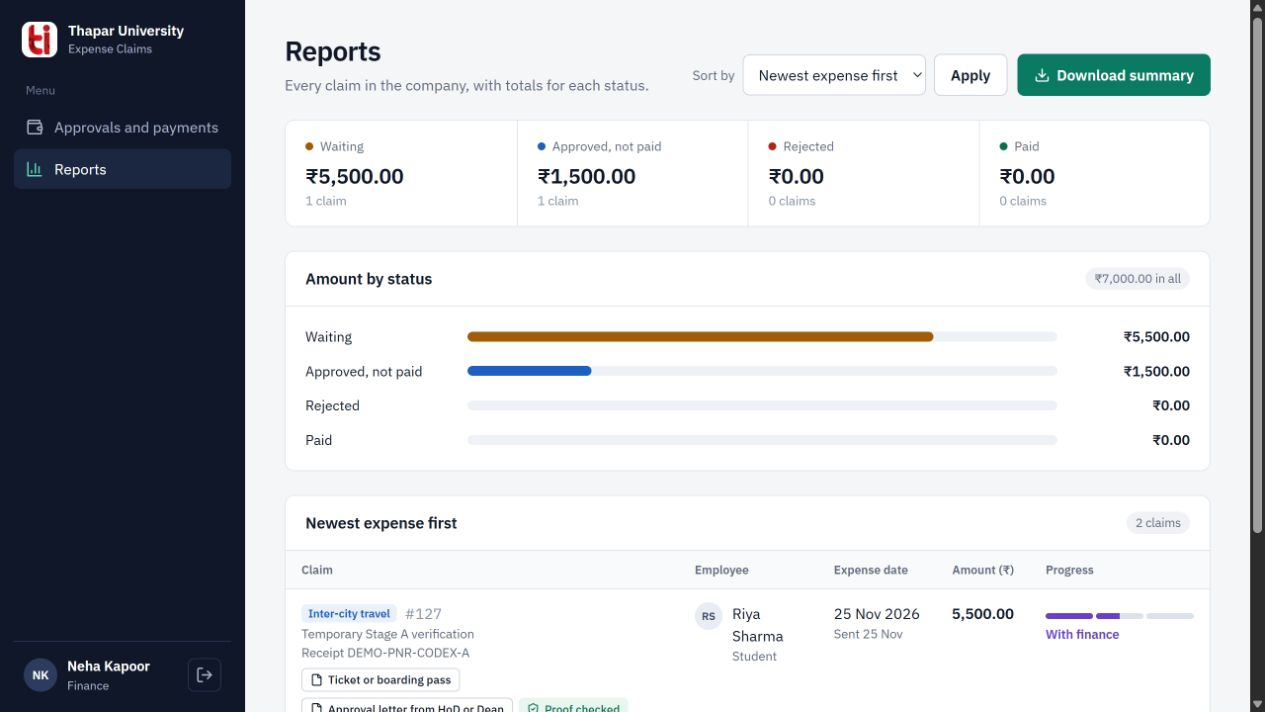
\includegraphics[width=\linewidth]{images/current-reports.jpg}
\caption{Thapar finance report with claim totals by status}
\end{figure}

\begin{figure}[H]
\centering
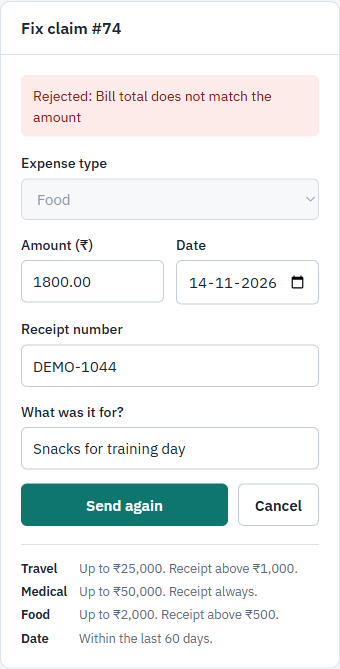
\includegraphics[width=0.42\linewidth]{images/resubmit.png}
\caption{Earlier demo showing how a claimant fixes a rejected claim}
\end{figure}

\section{Input and Output Demonstrations}

\textbf{Submitting a claim.} In an earlier demo, an employee submitted a travel claim of Rs 1,500 with receipt DEMO-2001. The application saved it and displayed a confirmation. The current travel form also requires a ticket attachment.

\begin{figure}[H]
\centering
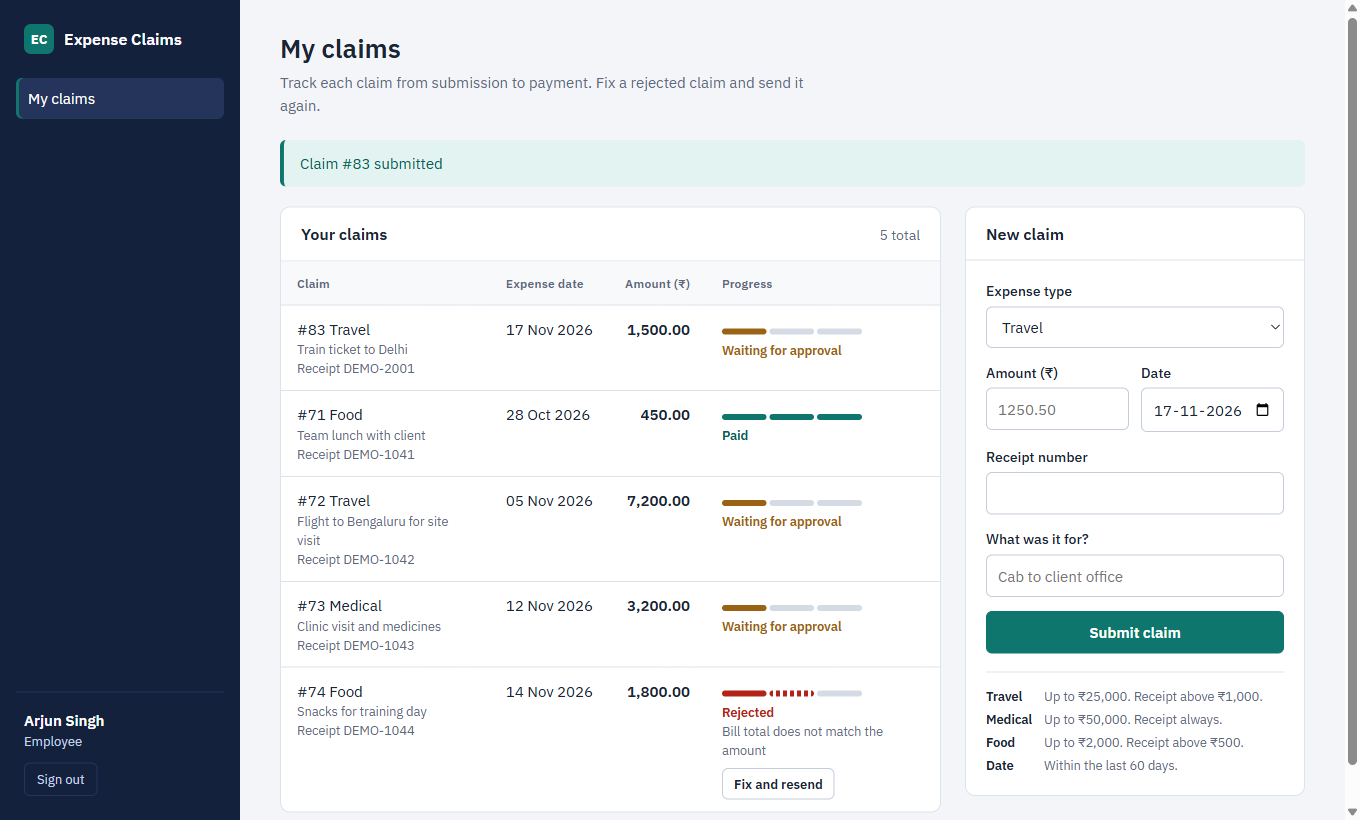
\includegraphics[width=\linewidth]{images/submit-success.png}
\caption{Claim submitted successfully}
\end{figure}

\textbf{Manager approval and payment.} The manager approves the claim with a note. Since it is below Rs 5,000 it becomes APPROVED directly. Finance then marks it as paid.

\begin{figure}[H]
\centering
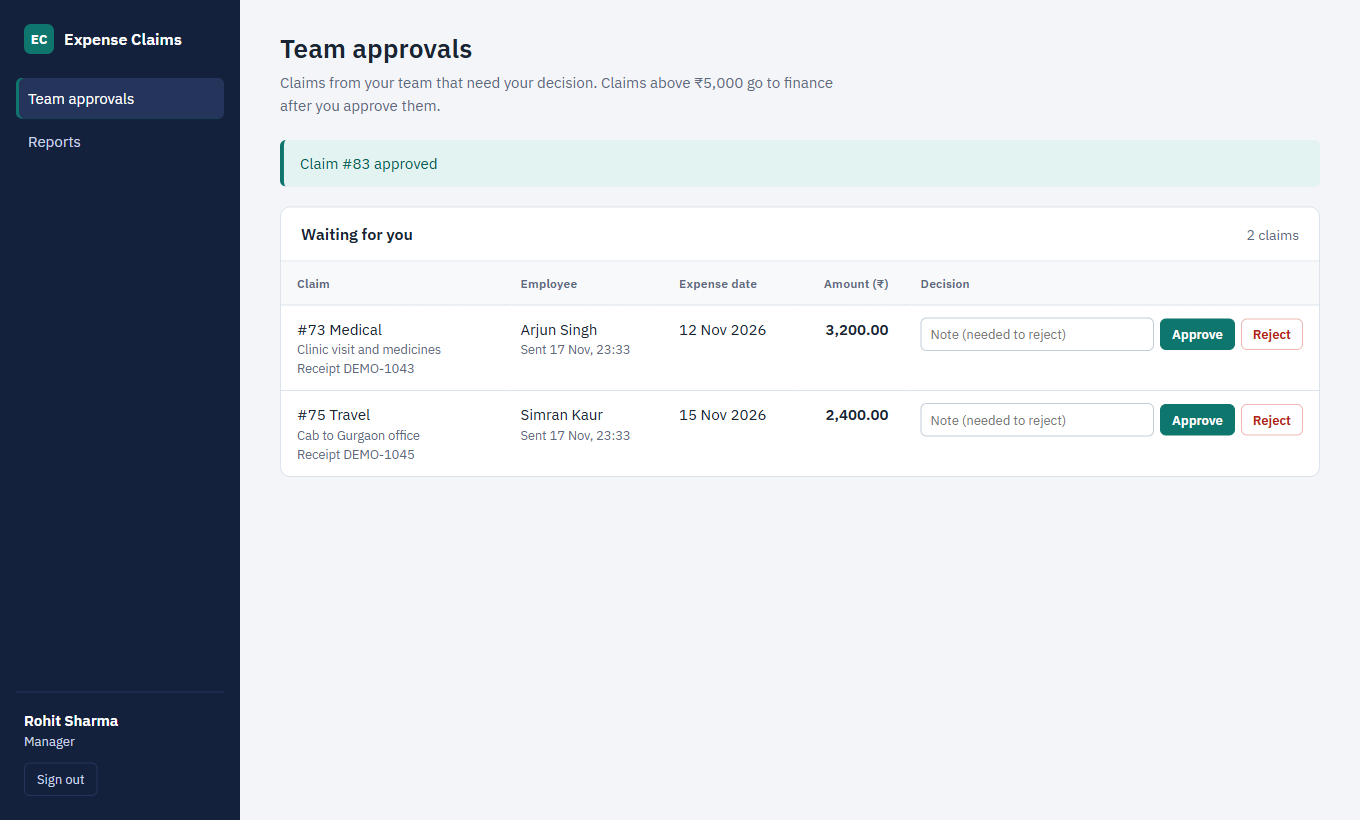
\includegraphics[width=\linewidth]{images/manager-approved.png}
\caption{Manager approves the claim}
\end{figure}

\begin{figure}[H]
\centering
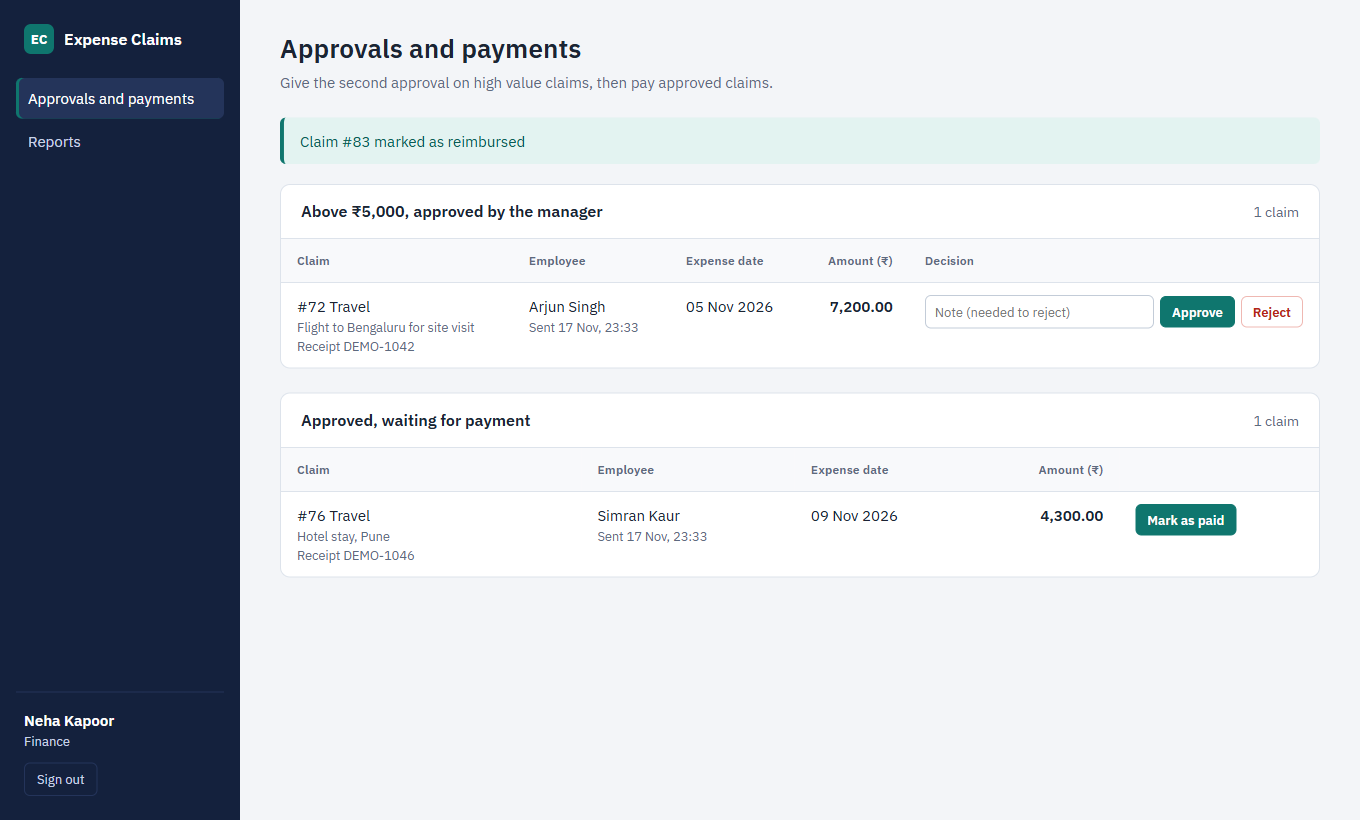
\includegraphics[width=\linewidth]{images/finance-paid.png}
\caption{Finance marks the claim as paid}
\end{figure}

\textbf{Downloaded summary file.} The file below was written with \texttt{FileWriter} and downloaded from the reports page by the finance user, sorted by status.

\lstinputlisting[language={},basicstyle=\ttfamily\scriptsize,caption={Summary file written with FileWriter}]{summary-sample.txt}

\textbf{Test results.} All 132 JUnit tests passed with \texttt{mvn test} against the local MySQL database. Signup used a test mailer.

\begin{table}[H]
\centering
\small
\begin{tabularx}{\linewidth}{>{\raggedright\arraybackslash}p{5.4cm} r Y}
\toprule
\textbf{Test class} & \textbf{Tests} & \textbf{What it checks}\\
\midrule
ClaimTest & 12 & Shared rules: amount, decimals, date window, lengths, lifecycle message\\
TravelClaimTest, MedicalClaimTest, FoodClaimTest, NewClaimTypesTest & 17 & Grade-specific limits, invoices and the equipment category\\
ClaimStatusTest & 4 & All 16 status pairs, only 4 moves allowed\\
ClaimServiceTest & 21 & Submission, resubmission, proof validation and type restrictions\\
ApprovalServiceTest & 24 & Escalation, proof confirmation, role checks and organisation isolation\\
ReportServiceTest & 13 & Role filtering, sorting, totals and file export\\
LoginServiceTest & 5 & Credential validation and compatibility with demo hashes\\
SignupServiceTest & 2 & Thapar email restriction and one-use signup code\\
AuthFilterTest, ClaimFormTest, MessagesTest, ErrorServletTest & 20 & Role rules, form parsing, error headings, error page text\\
JdbcClaimDAOTest, JdbcEmployeeDAOTest, JdbcProofDAOTest, DBConnectionTest & 14 & MySQL connectivity and storage for accounts, claims, proofs and audits\\
\midrule
\textbf{Total} & \textbf{132} & \\
\bottomrule
\end{tabularx}
\caption{JUnit test results}
\end{table}

\section{Error Handling Demonstrations}

\begin{figure}[H]
\centering
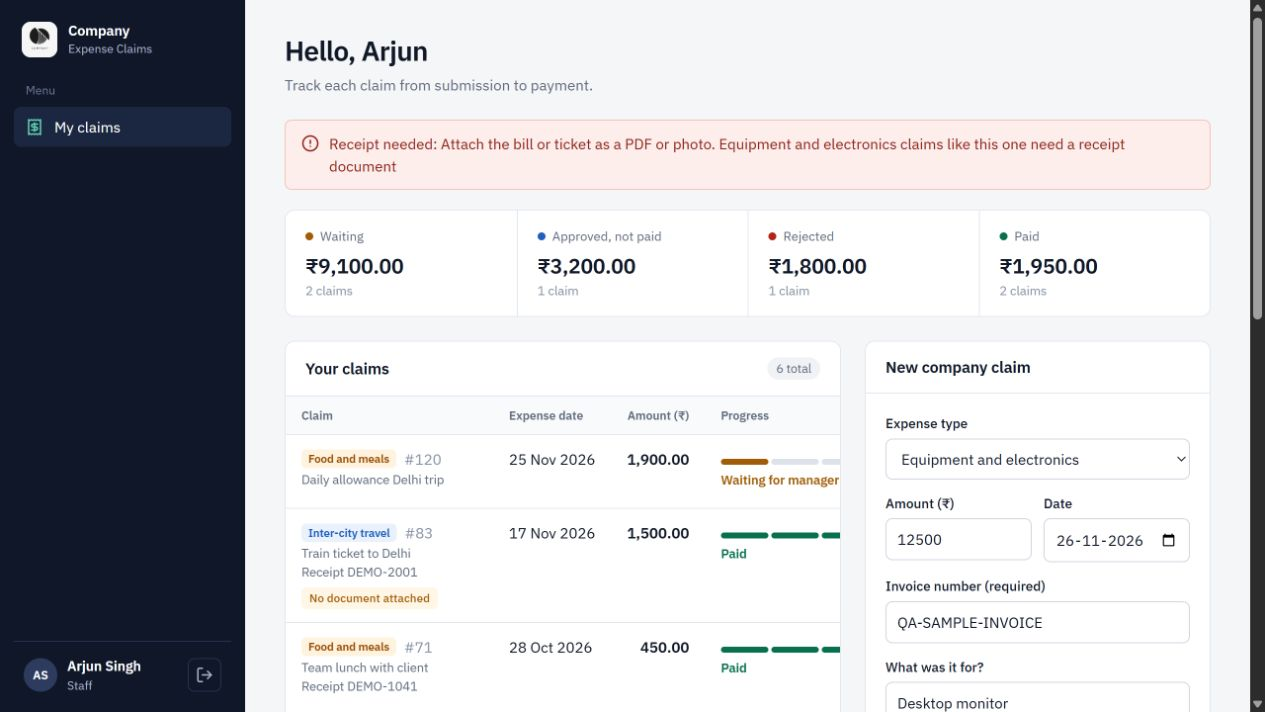
\includegraphics[width=\linewidth]{images/current-invoice-error.jpg}
\caption{Equipment claim rejected because the purchase invoice file is missing}
\end{figure}

\begin{figure}[H]
\centering
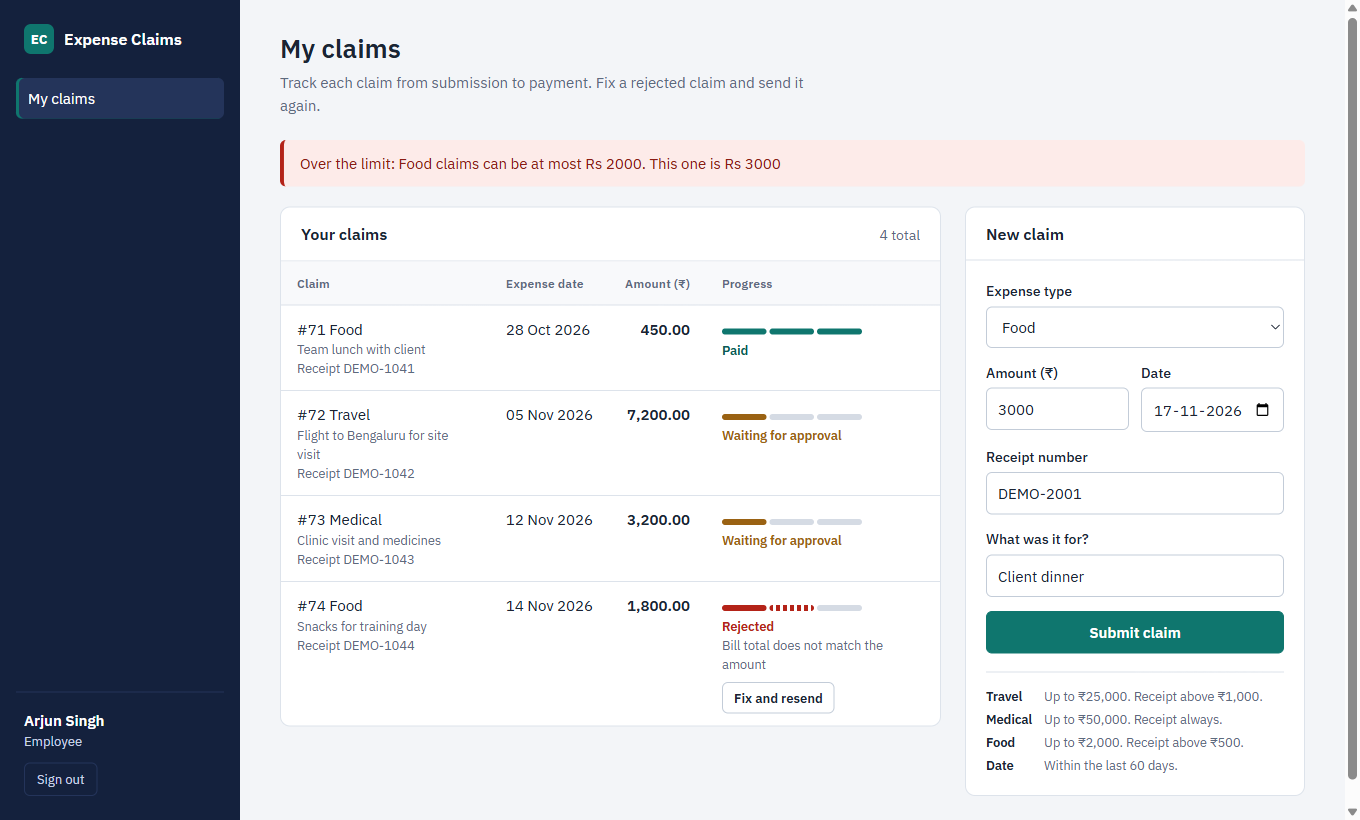
\includegraphics[width=\linewidth]{images/error-limit.png}
\caption{Earlier demo of a claim above the food limit. The form keeps the typed values}
\end{figure}

\begin{figure}[H]
\centering

\includegraphics[width=0.85\linewidth]{images/error-receipt.png}\\[6pt]

\includegraphics[width=0.85\linewidth]{images/error-duplicate.png}\\[6pt]

\includegraphics[width=0.85\linewidth]{images/error-not-allowed.png}\\[6pt]

\includegraphics[width=0.85\linewidth]{images/error-reason.png}
\caption{From top: missing receipt, duplicate receipt, opening another employee's claim by changing the URL, and rejecting without a reason}
\end{figure}

\begin{figure}[H]
\centering
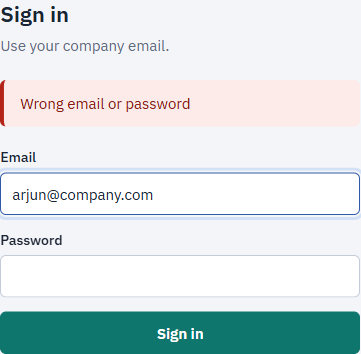
\includegraphics[width=0.42\linewidth]{images/login-error.png}
\caption{Wrong password}
\end{figure}

\begin{figure}[H]
\centering
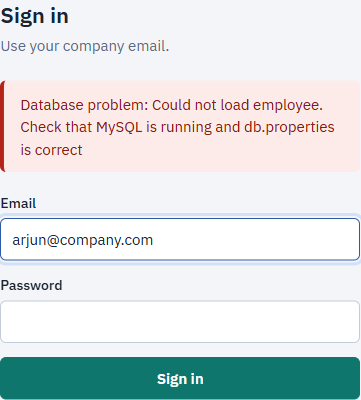
\includegraphics[width=0.42\linewidth]{images/error-database.png}
\caption{Signing in while MySQL is stopped (DataAccessException)}
\end{figure}

\textbf{Error pages.} \texttt{web.xml} sends every error status and every uncaught exception to \texttt{ErrorServlet}, which shows a styled page instead of the server's default one. Figure~\ref{fig:error403} shows the page an employee gets when they type the finance page address. Unknown addresses get a 404 page, and a server error gets a 500 page.

\begin{figure}[H]
\centering
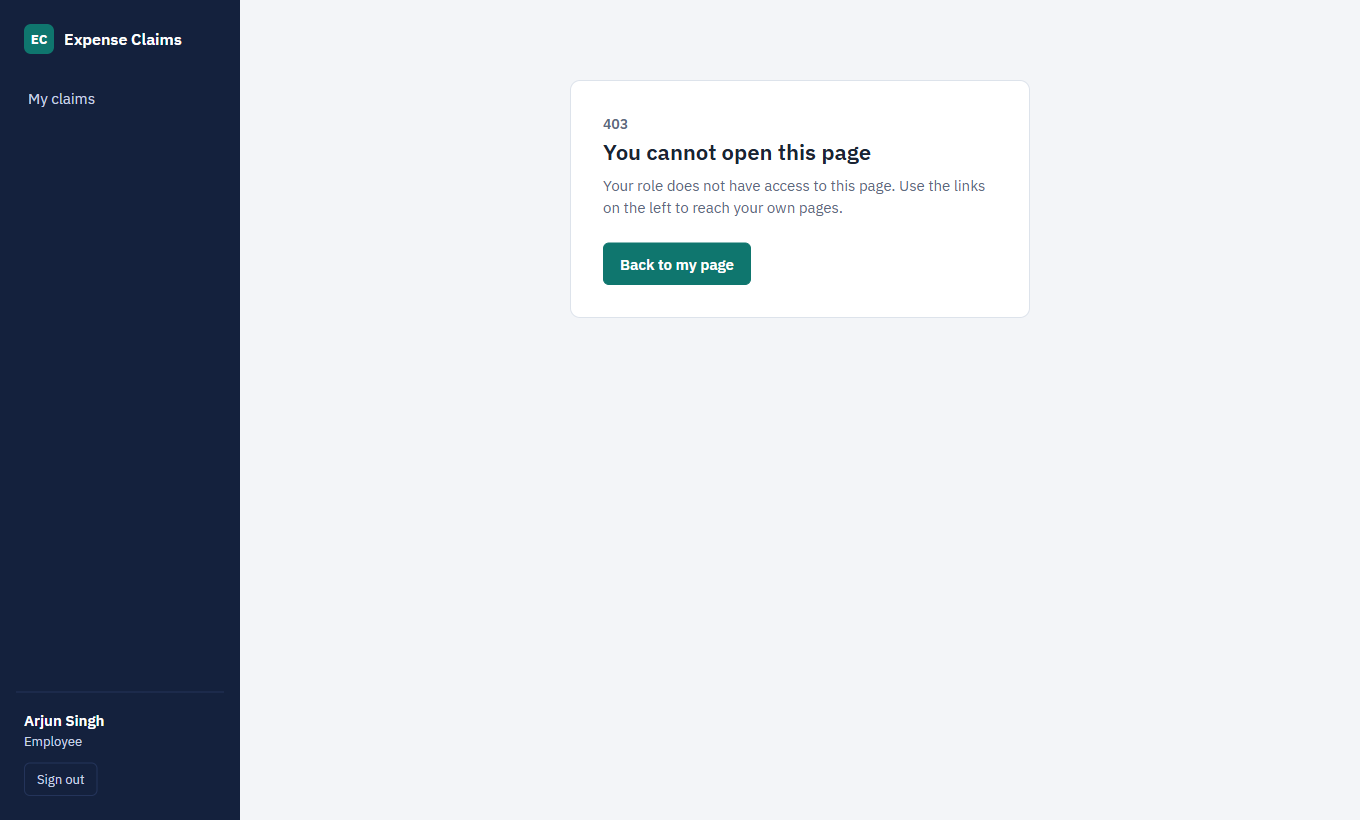
\includegraphics[width=\linewidth]{images/error-403.png}
\caption{403 page when an employee opens the finance page}
\label{fig:error403}
\end{figure}

Self approval cannot be shown on screen, because the pages never list a user's own claims. It is still blocked in \texttt{ApprovalService} and covered by the test \texttt{ownClaimCannotBeApproved} in \texttt{ApprovalServiceTest}.

% ---------------- References ----------------
\chapter*{References}
\addcontentsline{toc}{chapter}{References}

\begin{enumerate}[label={[\arabic*]}]
  \item H. Schildt, \textit{Java: The Complete Reference}, 12th ed., McGraw Hill, 2021.
  \item E. Gamma, R. Helm, R. Johnson and J. Vlissides, \textit{Design Patterns: Elements of Reusable Object-Oriented Software}, Addison-Wesley, 1994.
  \item D. Alur, J. Crupi and D. Malks, \textit{Core J2EE Patterns: Best Practices and Design Strategies}, 2nd ed., Prentice Hall, 2003 (Data Access Object pattern).
  \item Oracle, \textit{Java SE 21 API Documentation}. \url{https://docs.oracle.com/en/java/javase/21/docs/api/}
  \item Eclipse Foundation, \textit{Jakarta Servlet Specification 6.0}. \url{https://jakarta.ee/specifications/servlet/6.0/}
  \item The Apache Software Foundation, \textit{Apache Tomcat 10.1 Documentation}. \url{https://tomcat.apache.org/tomcat-10.1-doc/}
  \item The Thymeleaf Team, \textit{Tutorial: Using Thymeleaf 3.1}. \url{https://www.thymeleaf.org/documentation.html}
  \item Oracle, \textit{MySQL 8.0 Reference Manual} and \textit{MySQL Connector/J Developer Guide}. \url{https://dev.mysql.com/doc/}
  \item The JUnit Team, \textit{JUnit 5 User Guide}. \url{https://junit.org/junit5/docs/current/user-guide/}
  \item The Apache Software Foundation, \textit{Apache Maven Documentation}. \url{https://maven.apache.org/guides/}
  \item Resend, \textit{Send Email API}. \url{https://resend.com/docs/api-reference/emails/send-email}
  \item OWASP Foundation, \textit{OWASP Top 10} (broken access control, injection, cross site scripting). \url{https://owasp.org/www-project-top-ten/}
\end{enumerate}

\end{document}
